\documentclass[english, 11pt]{article}
\usepackage{notes}
\usepackage[colorinlistoftodos]{todonotes}
\usepackage{tikz}
\usepackage{pgfplots}
\usepackage{cancel}
\usepackage{wasysym}
%\renewcommand{\sfdefault}{cmss}
%\renewcommand{\familydefault}{\sfdefault}

\newcommand{\thiscoursecode}{MATH 237}
\newcommand{\thiscoursename}{Calculus III}
\newcommand{\thisprof}{Dr. Joseph West}
\newcommand{\me}{Liam Horne}
\newcommand{\thisterm}{Fall 2013}
\newcommand{\website}{LIHORNE.COM}
\usepackage{xcolor}
% Headers
\chead{\thiscoursename}
\lhead{\thisterm}

\newcommand{\boundellipse}[3]% center, xdim, ydim
{(#1) ellipse (#2 and #3)
}


%%%%% TITLE %%%%%
\newcommand{\notefront} {
\pagenumbering{roman}
\begin{center}

{\ttfamily \url{\website}} {\small}

\textbf{\Huge{\noun{\thiscoursecode}}}{\Huge \par}

{\Large{\noun{\thiscoursename}}}\\ \vspace{0.1in}

\vspace{0in}
\includegraphics[scale=0.5]{logo.png}

  {\noun \thisprof} \ $\bullet$ \ {\noun \thisterm} \ $\bullet$ \ {\noun {University of Waterloo}} \\

  \end{center}
  }

%   ooooo      ooo   .oooooo.   ooooooooooooo oooooooooooo  .oooooo..o
%   `888b.     `8'  d8P'  `Y8b  8'   888   `8 `888'     `8 d8P'    `Y8
%    8 `88b.    8  888      888      888       888         Y88bo.
%    8   `88b.  8  888      888      888       888oooo8     `"Y8888o.
%    8     `88b.8  888      888      888       888    "         `"Y88b
%    8       `888  `88b    d88'      888       888       o oo     .d8P
%   o8o        `8   `Y8bood8P'      o888o     o888ooooood8 8""88888P'


\begin{document}

  % Notes front
  \notefront
  % Table of Contents and List of Figures
  \tocandfigures
  % Abstract

  \doabstract{These notes are intended as a resource for myself; past, present, or future students of this course, and anyone interested in the material. The goal is to provide an end-to-end resource that covers all material discussed in the course displayed in an organized manner. If you spot any errors or would like to contribute, please contact me directly.}

  \section{Function of Several Variables}

  So far we've primarily seen functions of one variable. For example, some function $f$ usually has one input $x$ that outputs a unique result $f(x)$. Now, we'll look at functions $g$ that take some $(x,y)$ and produce a unique output $f(x,y,z)$. In general,
  $$(x_1, \cdots, x_n) \longrightarrow f \longrightarrow f(x_1, \cdots, x_n)$$

  \begin{defn}
    A \textbf{scalar function} is a function $f(x,y)$ is a rule which assigns each ordered pair $(x,y)$ in the set $D \subseteq \R^2$ a unique real number $z = f(x,y)$. $D$ is called the \textbf{domain} of $f$. The set $\{f(x,y) | (x,y) \in D\}$ is called the \textbf{range}.
  \end{defn}
  \begin{center}
    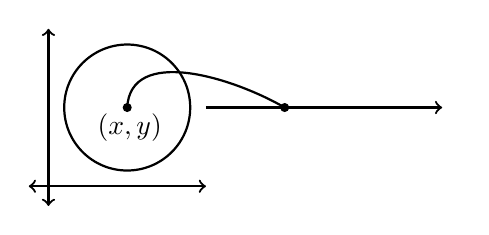
\begin{tikzpicture}
      \draw [<->, thick] (0,-0.25) --(0,2);
      \draw [<->, thick] (-0.25,0) --(2,0);
      \draw[thick] (1,1) circle(0.8cm);
      \draw[fill] (1,1) circle [radius=0.05];
      \node [right] at (.5,.75) {$(x,y)$};
      \draw [thick] (1,1) to [out=87,in=150] (3,1);
      \draw [->, thick] (2,1) --(5,1);
      \node [right] at (5,1) {$\Z$};
      \draw[fill] (3,1) circle [radius=0.05];
    \end{tikzpicture}
  \end{center}
  There is a similar definition for $f(x_1, \cdots, x_n)$. (See course notes)

  \begin{exmp}
    Consider the function $f(x,y) = 3x + 4y + 5$. Then $f(1,1) = 3 + 4 + 5 = 12$. The domain $D = \R^2$ and the range is $\R$.
  \end{exmp}

  \begin{exmp}
    Wind chill index with $T$ temperature C${}^{\circ}$ and $v$ wind speed in km/hr.
    \[ W(T, v) = 13.12 + 0.6215T - 11.37v^{0.16} + 0.3965Tv^{0.16} \]
    Thus for temperature $T = -10$ C${}^{\circ}$ and $v = 20$ we find the wind chill to be $-18$.
  \end{exmp}

  \section {Interpretations of $f(x,y)$}

  \begin{itemize}
    \item[]  \textbf {Geometrical}
    Consider a function $f : \R^2 \rightarrow \R$, this can be understood as a point on a plane consisting of the $x$ and $y$ axis, that maps to a single value on the $z$ plane. Visually, you can see the function $f$ turn points on a plane to a surface relative to $z$.

    \item[] \textbf {Physical}
    Some examples include the temperature at $(x,y)$ like in Example 2. Others include calculating the density of 3-dimensional object at the point $(x,y)$, or the pressure, etcetera.

  \end{itemize}

  \begin{exmp}
    Consider the function $f(x,y) = 16 - x^2 - 4y^2$. The domain is all of $\R^2$ and the range is $\R_{\geq 16}$ since having domain restricted to $\R^2$ means the squared terms will always be greater than 0.
  \end{exmp}

  \begin{defn}[level curve]\label{level curve}
    The \textbf{level curves} of $f(x,y)$ are the curves in $\R^2$ with the equation $f(x,y) = k$ where $k$ is a constant in the range of $f$.
  \end{defn}

  Returning to our example, $16 - x^2 - 4y^2 = k$ is the equation for our level curves. Rearranging gives $x^2 + 4y^2 = 16 - k$ for $k \in \R_{\leq 16}$; this is a family of ellipses. \\
  $k = 0 \implies x^2 + 4y^2 = 16$ \\
  $k = 4 \implies x^2 + 4y^2 = 12$ \\
  $k = 8 \implies x^2 + 4y^2 = 8$ \\
  $k = 12 \implies x^2 + 4y^2 = 4$ \\
  $k = 16 \implies x^2 + 4y^2 = 0$
  \begin{center}
    Refer to \textbf{Graph 1.1}
  \end{center}

  Our surface looks like $z = 16 - x^2 - 4y^2$3

   \begin{center}
    Refer to \textbf{Graph 1.2}
   \end{center}

  \begin{exmp}
    $f(x,y) = x^2 - y^2$. The Level curves: $x^2 - y^2 = k$ is a family of hyperbolas. Note that $k = 0 \implies x^2 = y^2 \implies y = \pm x$. Additionally, as an aside note that $y = \pm \sqrt{x^2 - k} \approx \pm \sqrt{x^2}$ for large $x$.

     \begin{center}
     Refer to \textbf{Graph 1.3, 1.4}
     \end{center}

    Now we plot the \textbf{cross-sections} of $z = f(x,y)$ using $z = x^2 - y^2$. (here he plots two regular 2d graphs, one for y-z, one for x-z using $z = c^2 - y^2$ and $z = x^2 - d^2$ for various values of $c$ and $d$. \\ Finally the surface can be drawn, it looks like a "Saddle Surface".

     \begin{center}
    Refer to \textbf{Graph 1.5}
  \end{center}
  \end{exmp}



\begin{exmp}
  $z = f(x,y) = \sqrt{4-x^2-y^2}$. The domain is $\{ (x,y) | x^2 + y^2 \leq 4 \}$ which is just a circle of radius 2 centered at the origin. The range is $0 \leq z \leq 2$. \\
  The level curves are described by $\sqrt{4-x^2-y^2} = k$ for $k \in [0,2] \implies x^2 + y^2 = 4-k^2$ (circles). \\
  The cross-sections can be examined so
  \[ x = c \implies z = \sqrt{4-c^2-y^2} \implies y^2 + z^2 = 4-c^2 \]
  with $z \geq 0$ (semicircles). It is often the case that $x$ and $y$ have symmetry, such that replacing $x$ with $y$ in the last step would produce the same cross-sections with the $x$ axis swapped with the $y$. The surfaces of this graph look like a hemisphere. It's a sphere of radius $R$ centered at origin: $x^2 + y^2 + z^2 = R^2$ with $R = 2$.

 \begin{center}
    Refer to \textbf{Graph 1.6}
  \end{center}

\end{exmp}

\begin{defn}
  A \textbf{quadratic surface} is $Ax^2 + By^2 + Cz^2 + Dxy + Ey^2 + Fx^2 + Gx +Hy + Iz +J = 0$
\end{defn}

\begin{exmp}
  Sketch $\frac{x^2}{4} + y^2 - \f{z^2}{4} = 1$ (implicity defined surface). The level curves where $z = k$ are
  \[ \frac{x^2}{4} + y^2 - \f{k^2}{4} = 1 \implies \f{x^2}{4} + y^2 = 1 + \f{k^2}{4} \]
  The cross-sections where $x = c$ refer to
  \[ y^2 - \f{z^2}{4} = 1 - \f{c^2}{4} \]
  \begin{center}
     Refer to \textbf{Graphs 1.7 - 1.9}
     \end{center}
\end{exmp}
The generalized term for level curves is \textbf{level sets}, so for example the level sets of $f(x,y,z) = k$ are a family of surfaces (level surfaces).

\section{Limits}

\begin{notation}
  We'll represent a point in $\R^n$ as $\vx$. For example in $\R^2$, $\vx = (x^{(1)},x^{(2)})$ and in general
  \[ \vx = (x^{(1)}, \cdots, x^{(n)}) \]
\end{notation}

Recall that in first year we looked at limits for $x \in \R$, so there were only two sides to a limit to check for consistency. They were $\lim_{x \rightarrow a^-} f(x)$ and $\lim_{x \rightarrow a^+} f(x)$. For functions of multiple variables, there are infinitely many directions to check for this consistency.

\begin{defn}[neighbourhood]\label{neighbourhood}
  A \textbf{neighbourhood} of $\va \in \R^2$ of radius $r > 0$ is a subset of $\R^2$ defined by
  \[ N_r(\va) = \{ \vx \in \R^2 \ | \  ||\vx - \va|| < r \} \]
\end{defn}

For simplicity we will mostly deal with functions of the form $f : \R^2 \rightarrow \R$, thus our limit definition will be defined for these too.

\begin{defn}
  Suppose $f(x,y)$ is defined in some neighbourhood of $\va$, except possibly at $\va$. If for every $\epsilon > 0$ there exists a $\delta > 0$ such that
  \[ ||\vx - \va|| < \delta \implies |f(\vx) - L| < \epsilon \]
  then we say that "the limit as $\vx$ approaches $\va$ exists and equals L" and we write
  \[ \lim_{(\vx \rightarrow \va)} f(x) = L \]
\end{defn}

 \begin{center}
    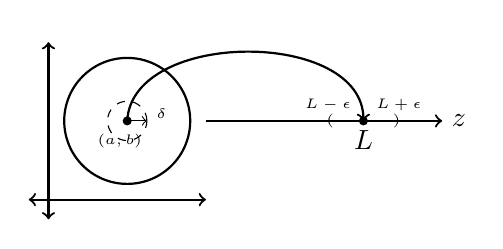
\begin{tikzpicture}
      \draw [<->, thick] (0,-0.25) --(0,2);
      \draw [<->, thick] (-0.25,0) --(2,0);
      \draw [->] (1,1) -- (1.25,1);
      \draw[thick] (1,1) circle(0.8cm);
      \draw[fill] (1,1) circle [radius=0.05];
      \draw[dashed] (1,1) circle [radius=0.25];
      \node [below, right] at (.5,.75) {\tiny $(a,b)$};
      \node [above right] at (1.25,0.9) {\tiny $\delta$};
      \draw [thick, ->] (1,1) to [out=87,in=90] (4,1);
      \draw [->, thick] (2,1) --(5,1);
      \node [right] at (5,1) {$z$};
      \draw[fill] (4,1) circle [radius=0.05];
      \node [below] at (4,1) {$L$};
      \node [above] at (4.45,1) {\tiny{$L+\epsilon$}};
      \node [above] at (3.55,1) {\tiny{$L-\epsilon$}};
      \node [left] at (3.75,1) {\tiny $($};
      \node [right] at (4.25,1) {\tiny $)$};
    \end{tikzpicture}
  \end{center}

\textbf{Proving that a limit does not exist}

To prove that \textbf{a limit does not exist}, the key idea is to show that different limits are reached along different paths.

  \begin{exmp}
    Show that the following limit does not exist
    \[ \lim_{(x,y) \rightarrow (0,0)} \f{x^2-y^2}{x^2+y^2} \]
    Look at the value of $f$ along straight lines through the origin as $(x,y) \rightarrow (0,0)$.
    \[ \lim_{x \rightarrow 0} f(x,mx) = \lim_{x\rightarrow 0} \f{1-m^2}{1+m^2} \]
    Since this depends on $m$, the limit does not exist.
  \end{exmp}

  \begin{exmp}
    \[ \lim_{\vx \rightarrow \vzero} \f{2x^2 y^{\f{1}{3}}}{x^3 + y} \]
    Trying $y = mx$ still simplifies to a term containing $x$ thus goes to 0. Thus, we try a cubic function of $x$; $y = x^3$. So,
    \[ lim_{x\rightarrow 0} f(x,x^3) = \lim_{x\rightarrow 0}\f{2x^2(x^3)^{\f{1}{3}}}{x^3 + x^3} = 1 \]
    Since this limit is not unique for different curved approaching the same point, this limit does not exist.
  \end{exmp}

  \begin{exmp}
    Show that
    \[ \lim_{(x,y)\rightarrow(1,0)} \f{x^2 - y - 1}{x + y - 1} \]
    does not exist. We could try $y = m(x-1)$, or even easier, we will try the vertical line $x = 1$:
    \[ \lim_{y\rightarrow0}f(1,y) = \lim_{y\rightarrow 0} \f{1 - y - 1}{1 + y - 1} = -1\]
    Similarly along the horizontal line $y = 0$ we get
    \[ \lim_{x\rightarrow1}f(x,1) = \lim_{x\rightarrow 1} \f{x^2 - 1}{x - 1} = \lim_{x\rightarrow 1} \f{(x-1)(x+1)}{x-1} = 2\]
    Since the limits are different, we have shown that the limit does not exist.
  \end{exmp}

  \textbf{Proving that a limit does exist}

  \begin{thrm}[squeeze theorem]\label{squeeze}
    If there exists a $B(x,y)$ such that
    \[ |f(x,y) - L| \leq B(x,y) \]
    for all $(x,y)$ in some neighbourhood of $(a,b)$ except possibly at $(a,b)$ and
    \[ \lim_{(x,y) \rightarrow (a,b)} B(x,y) = 0 \mbox{ \ \ \ then \ \ \ } \lim_{(x,y) \rightarrow (a,b)} f(x,y) = L\]
  \end{thrm}

  \begin{proof}
    Since $\lim_{(x,y)\rightarrow(a,b)} B(x,y) = 0$, there exists a $\delta > 0$ such that $|B(x,y) - 0| < \epsilon$ whenever $ ||(x,y)-(a,b)|| < \delta $ for any $\epsilon > 0$ by the definition of a limit. Then, $|f(x,y) - L| \leq |B(x,y)| < \epsilon$
    whenever $||(x,y) - (a,b)|| < \delta$. So by the definition of a limit,
    \[ \lim_{(x,y)\rightarrow(a,b)}f(x,y) = L \]
  \end{proof}

  \begin{exmp}
    Show that
    \[ \lim_{(x,y)\rightarrow(0,0)}\f{2x^2y}{x^2 + y^2} = 0. \]
    First we consider
    \begin{align*}
      |f(x,y) - L| & = \left| \f{2x^2y}{x^2+y^2} - 0 \right| \\
                   & = \f{2x^2|y|}{x^2+y^2} \\
                   & \leq \f{(2x^2 + 2y^2)|y|}{x^2+y^2} \\
                   & = 2|y|
    \end{align*}
    So we choose $B(x,y) = 2|y|$. Now, clearly we see that
    \[ \lim_{(x,y)\rightarrow(0,0)} 2|y| = 0 \]
    Now, by the \nameref{squeeze} (since $0 \leq f(x,y) \leq B(x,y)$)
    \[ \lim_{(x,y)\rightarrow(0,0)} \f{2x^2y}{x^2+y^2} = 0 \]
  \end{exmp}

  \begin{exmp}
    Evaluate
    \[ f(x,y) = \lim_{(x,y)\rightarrow(0,0)} \f{x^4 + x^2 + y^4 + y^2}{x^2 + y^2} \]
    or show that it does not exist. First we try to prove that it does not exist, so we will test the lines $y = mx$. Then,
    \[ f(x,mx) = \f{x^4+x^2+(mx)^4+(mx)^2}{x^2 + (mx)^2} = \f{x^2((1+m^2)+x^2(1+m^4))}{x^2(1+m^2)} = 1 + x^2 \f{1+m^4}{1+m^2}\]
    So, $\lim_{x\rightarrow 0} f(x,mx) = 1 + 0 = 1$, thus the limit might be 1. Next, we try to show that the limit is 1; we try to find a function to use in conjuction with the squeeze theorem. Consider,
    \begin{align*}
      \left| \f{x^4+x^2+y^4+y^2}{x^2+y^2} - 1 \right| & = \left| \f{x^4+x^2+y^4+y^2-(x^2+y^2)}{x^2+y^2} \right| \\
             & = \f{x^4+y^4}{x^2+y^2}
    \end{align*}
    Note that
      \begin{align*}
        (x^2 + y^2)^2 & = x^4 + y^4 + 2x^2y^2 \implies x^4 + y^4 = (x^2 + y^2)^2 - 2x^2y^2 \leq (x^2 + y^2)^2
      \end{align*}
      So,
      \begin{align*}
        |f(x,y)-1| & = \f{x^4+y^4}{x^2+y^2} \\
        & \leq \f{(x^2+y^2)^2}{x^2+y^2} \\
        & = x^2 + y^2 \\
        & \rightarrow 0 \mbox { \ \ as $(x,y) \rightarrow (0,0)$}
      \end{align*}
  \end{exmp}

  \begin{rem} A few comments on inequality tricks (pg. 8 of course notes):
    \[ |x| = \sqrt{x^2} \leq \sqrt{x^2 + y^2} \]
    \begin{align*}
       (|x|-|y|)^2 & \geq 0 \\
       x^2 - 2|x||y| + y^2 & \geq 0 \\
       2|x||y| & \leq x^2 + y^2
     \end{align*}
     And some Limit theorems (pg. 10 of course notes):
     \[ \mbox{e.g., } \lim_{x\rightarrow0} f(x) + g(x) = \lim_{x\rightarrow0} f(x)+ \lim_{x\rightarrow0} g(x) \]
  \end{rem}
  %%%%%%%%%%%%%%%%%%%%%%%%%%%%%%%%%%%%%%%%%%%%%%%

  \section{Continuous Functions}

  \begin{defn}[continuous]\label{continuous}
    A function $f(x,y)$ is \textbf{continuous} at $(a,b)$ if and only if
    \[ \lim_{(x,y)\rightarrow(a,b)} f(x,y) = f(a,b) \]
    and $f$ is \textbf{continuous} on $D \subseteq \R^2$ if it is continuous at every point in $D$.
  \end{defn}

  \begin{exmp}
    Let $f(x,y) = \f{x^4+x^2+y^4+y^2}{x^2+y^2}$, $(x,y) \not = (0,0)$. \\
    Earlier we showed that
    \[ \lim_{(x,y)\rightarrow(0,0)} f(x,y) = 1 \]
    If we define $f(0,0) = 1$, then $f$ would be \nameref{continuous} at $(0,0)$.
  \end{exmp}

  \begin{exmp}
    Let
    \[ f(x,y) = \piecewise{\f{\sin(x^2 + 2y^2)}{x^2+y^2}}{if $(x,y) \not = (0,0)$}{k}{if $(x,y) = (0,0)$} \]
    Can we define $k$ to make $f$ \nameref{continuous} at $(0,0)$?\\
    This requires showing that the following limit exists
    \[ \lim_{(x,y)\rightarrow(0,0)} \f{\sin(x^2+2y^2)}{x^2+y^2} \]
    Consider the lin $y = 0$, then we find that the limit goes to 1, and for the line $x=0$ we fine the line goes to 2, therefore the limit does not exists. So, no such $k$ exists to satisfy the function's continuity.
  \end{exmp}

  \begin{defn}[continuity theorem]\label{continuitytheorem}
    Let $f$ and $g$ be \nameref{continuous} at $(a,b)$. Then
    \begin{itemize}
      \item[(1)] $f+g$ and $fg$ are \nameref{continuous} at $(a,b)$.
      \item[(2)] $\f{f}{g}$ is \nameref{continuous} at $(a,b)$ for $g(a,b) \not = 0$.
    \end{itemize}
  \end{defn}

  \begin{defn}[composition of functions]\label{composition}
  Suppose $f : \R \rightarrow \R$ and $g : \R^2 \rightarrow \R$, then
    \[ (f\circ g)(x,y) = f(g(x,y)) \]
  \end{defn}

  \begin{defn}[Continuity of Composition Theorem]
    Let $f$ be a function of one variable and $g$ be a function of two variables. Then, if $g$ is \nameref{continuous} at $(a,b)$ and $f$ is \nameref{continuous} at $g(a,b)$ then $f\circ g$ is \nameref{continuous} at $(a,b)$.
  \end{defn}

  \begin{exmp}
    Consider $f(x,y) = \f{y\sin x - \cos y}{x^2+y^2}$, since $f$ is quotient of two \nameref{continuous} functions, by the \nameref{continuitytheorem} the function $f$ is \nameref{continuous} at all points in $\R^2$ except $(0,0)$ (since $x^2 + y^2 = 0$ at $(0,0)$).
  \end{exmp}

  \begin{exmp}
    Consider the function $e^{x^3 - \sin(xy)}$.
    Clearly it is \nameref{continuous} everywhere by the \nameref{continuitytheorem}.
  \end{exmp}

  \begin{exmp}
    Evaluate
    \[ \lim_{(x,y)\rightarrow(0,0)} \f{e^{x^2} + \ln(2+y^2+x^4)}{(x-1)^2 + y^4} \]
    Plugging in $(0,0)$ gives us the result, $1+\ln(2)$; which we can do since the function is \nameref{continuous} at $(0,0)$ by the \nameref{continuitytheorem}s.
  \end{exmp}

  \begin{exmp}
    Determine where the following function is \nameref{continuous}:
    \[ f(x,y) = \piecewise{\f{e^{xy} - 1}{x^2 + y^2}}{$(x,y) \not = (0,0)$}{0}{$(x,y)=(0,0)$} \]
  \end{exmp}

  For $(x,y) \not = (0,0)$, $f$ is \nameref{continuous} by the \nameref{continuitytheorem}s. Now, does
  \[ \lim_{(x,y) \rightarrow (0,0)} \f{e^{xy}-1}{x^2 + y^2} = 0 \]
  Checking along $x=0$ we find the limit to be 0, and checking along $y=x$ we find the limit to be
  \begin{align*}
    \lim_{x\rightarrow 0} \f{e^{x^2} -1}{2x^2} & = \lim_{x\rightarrow 0} \f{2xe^{x^2}}{4x} & \mbox{(L'hopital's Rule)} \\
    & = \f{1}{2} \\
    & \not = 0
  \end{align*}
  So, $f$ is \nameref{continuous} for all $(x,y) \not = (0,0)$, but it is not continuous at the origin.



  \begin{exmp}
    Determine where
    \[ f(x,y) = \piecewise{\f{x^4y^6}{x^6+y^{12}}}{$(x,y) \not = (0,0)$}{0}{$(x,y) = (0,0)$} \]
    is \nameref{continuous}. \\ At $(x,y) \not = (0,0)$ $f$ is \nameref{continuous} by \nameref{continuitytheorem}s. Now we check whether
    \[ \lim_{(x,y) \rightarrow (0,0)} \f{x^4y^6}{x^6+y^{12}} = f(0,0) = 0 \]
    We attempt to show the correctness of this limit by \nameref{squeeze}. We use the following rewrite
  \[  \left| \f{x^4y^6}{x^6+y^{12}} - 0 \right| = \f{(x^6)^{\f{2}{3}}(y^{12})^{\f{1}{2}}}{x^6+y^{12}} \]
  Then clearly we can show that
  \[  \f{(x^6)^{\f{2}{3}}(y^{12})^{\f{1}{2}}}{x^6+y^{12}} \leq \f{(x^6+y^{12})^{\f{2}{3}}(y^{12}+x^{6})^{\f{1}{2}}}{x^6 + y^{12}} \]
  So,
  \[  \left| \f{x^4y^6}{x^6+y^{12}} - 0 \right| \leq \f{(x^6 + y^{12} )^{\f{7}{6}}}{x^6 + y^{12}} = (x^6 + y^{12})^{\f{1}{6}} \longrightarrow 0 \mbox {\ as $(x,y) \rightarrow (0,0)$} \]
  Therefore by \nameref{squeeze},
  \[ \lim_{(x,y) \rightarrow (0,0)} \f{x^4y^6}{x^6+y^{12}} = 0  \]
  So, $f$ is continuous at $(0,0)$ by inspection.
  \end{exmp}

  % \begin{rem}
  %   Another way this example can be approached is to use the inequality
  %   \[ 2|a||b| \leq a^2 + b^2 \]
  %   Where we can think of $a = x^4$ and $b = y^6$ in the context of the example. So,
  %   \[ x^4y^6 \leq \f{1}{2}(x^8 + y^{12}) < \f{1}{2}(x^6 + y^{12}) \]
  % \end{rem}

  \section{The Linear Approximation}

  \textbf{Partial Derivatives}
  We now look at different ways to differentiate a function $f : \R^2 \rightarrow \R$. We consider two ways
  \begin{itemize}
    \item[1.] Hold $y$ fixed, differentiate with respect to $x$.
    \[ \f{\di f}{\di x} \]
    \item[2.]  Hold $x$ fixed, differentiate with respect to $y$.
    \[ \f{\di f}{\di y} \]
  \end{itemize}
  \begin{exmp}
    Differentiate $f(x,y) = y^2\sin(xy)$.
    \begin{align*}
      \f{\di f}{\di x}(x,y) & = y^2 \cos (xy) \cdot y \\
      \f{\di f}{\di y}(x,y) & = 2y\sin(xy) + y^2\cos(xy)\cdot x
    \end{align*}
    We simply treat the non-dependent variables as constants when differentiating. Now, evaluating at a point (e.g., $(1,\pi)$) we get
    \begin{align*}
      \f{\di f}{\di x}(1,\pi) & = \pi^2 \cos (\pi) \cdot \pi = -\pi^3\\
      \f{\di f}{\di y}(1,\pi) & = 2\pi\sin(\pi) + \pi^2\cos(\pi) = - \pi^2
    \end{align*}
  \end{exmp}

  \begin{notation}
    In this course we will use the following notation:
    \[ \f{\di f}{\di x} = f_x\]
    for any variable $x$.
  \end{notation}

  \begin{defn}[partial derivative]\label{partialderivative}
    The \textbf{partial derivatives} of $f(x,y)$ at $(a,b)$ are
    \begin{align*}
      \f{\di f}{\di x} (a,b)  &= \lim_{h \rightarrow 0} \f{f(a+h,b)-f(a,b)}{h} \\
      \f{\di f}{\di y} (a,b)  &= \lim_{h \rightarrow 0} \f{f(a,b+h) - f(a,b)}{h}
    \end{align*}
    provided that the limit exists.
  \end{defn}

  \begin{note}
    This definition can of course be expanded to $f : \R^n \rightarrow \R$.
  \end{note}

  \begin{exmp}
    Consider the function
    \[ f(x,y) = \piecewise{\f{x^3+y^4}{x^2+y^2}}{$(x,y) \not = (0,0)$}{0}{$(x,y) = (0,0)$} \]
    Find $f_x(0,0)$ and $f_y(0,0)$. \\
    We use the formal defintion of a \nameref{partialderivative},
    \begin{align*}
      f_x(0,0) & = \lim_{h \rightarrow 0} \f{f(0+h,0)-f(0,0)}{h} = \lim_{h \rightarrow 0} \f{\f{h^3+0}{h^2+0}-0}{h} = 1 \\
      f_y(0,0) & = \lim_{h \rightarrow 0} \f{f(0,0+h)-f(0,0)}{h} = \lim_{h \rightarrow 0} \f{\f{0+x^4}{0 +h^2}-0}{h} = 0
    \end{align*}
  \end{exmp}

  \begin{note}
    You must use the definition when the usual rules for differentiation don't apply.
  \end{note}

  \begin{exmp}
    Review Example 2 on page 29 of the course notes.
  \end{exmp}

  \begin{exmp}
     The volume of an ideal gas in $\mbox{cm}^3$ with pressure in atm and temperature in K is
     \[ V = \f{82.06T}{P} \]
     Find the rate of change of volume with respect to temperarture and with respect to pressure when $T = 300$ K and $P = 5$ atm.
     \begin{align*}
       \f{\di V}{\di T} &= \f{82.06}{P} \approx 16.41 \ \f{\mbox{cm}^3}{\mbox{K}} \\
       \f{\di V}{\di P} &= -82.06TP^{-2} \approx -984.72 \ \f{\mbox{cm}^3}{\mbox{atm}}
     \end{align*}
  \end{exmp}

  \begin{notation}
    Second partial derivatives can be written as
  \[ \f{\di}{\di x} \left( \f{\di f}{\di x} \right) = \f{\di^2 f}{\di x^2} = f_{xx} = D_1D_1f = D_1^2f \]
  with the operator notation,
  \[ D_1 = \f{\di}{\di x}, D_2 = \f{\di}{\di yz} \]
  So taking derivatives with respect to different variables can be shown as,
  \[ \f{\di}{\di y} \left( \f{\di f}{\di x} \right) = \f{\di^2 f}{\di y \di x} = f_{xy}= D_2D_1f \]
  and
  \[ \f{\di}{\di x} \left( \f{\di f}{\di y} \right) = \f{\di^2 f}{\di x \di y} = f_{yx}= D_1D_2f \]
  \end{notation}

  \begin{exmp}
    Find the second partials of $f(x,y) = x^2e^{-xy}$. The first are,
    \[ \f{\di f}{\di x} = 2xe^{-xy} - x^2ye^{-xy} \]
    \[ \f{\di f}{\di y} = -x^3e^{-xy} \]
    Then the seconds are,
    \[ f_{xx} = \f{\di}{\di x} \left( 2xe^{-xy} - x^2ye^{-xy} \right) = 2e^{-xy} - 4xye^{-xy} + x^2y^2e^{-xy}  \]
    \[ f_{xy} = -3x^2e^{-xy} + x^3ye^{-xy} \]
    \[ f_{yx} =3x^2e^{-xy} + x^3ye^{-xy} \]
    \[ f_{yy} = x^4e^{-xy} \]
    Note that the mixed partials are equivalent.
  \end{exmp}

  \begin{thrm}[Clairaut's Theorem]\label{clairaut}
    If $f_x$, $f_y$, $f_{xy}$, and $f_{yx}$ are all defined in some \nameref{neighbourhood} of $f_{xy}(x,y)$, and $f_{yx}(x,y)$ are \nameref{continuous} at $(a,b)$ then
    \[ f_{xy}(a,b) = f_{yx}(a,b) \]
  \end{thrm}

  \begin{defn}[Hessian Matrix]\label{hessian}
    \[ Hf(x,y) =  \left(\begin{matrix} f_{xx} & f_{xy} \\ f_{yx} & f_{yy} \end{matrix}\right) \]
  \end{defn}

  \begin{rem}
    There are $2^n$ $n$-partial-derivatives of a function $f(x,y)$. (e.g., 4 possible second derivates of $f(x,y)$)
  \end{rem}

  \begin{defn}[class]\label{class}
    $f \in C^k$ "$f$ is of class $C^k$" means that the $k^{th}$ \nameref{partialderivative}s of $f$ are \nameref{continuous}. For example, if $f$ is of class $C^2$ then $f_{xx},f_{xy},f_{yx},f_{yy}$ are \nameref{continuous}, so $f_{xy} = f_{yx}$ by \nameref{clairaut}.
  \end{defn}

  \begin{defn}[tangent plane]\label{tangentplane}
    The geometric interpreation of $f_x$ and $f_y$ is a \textbf{tangent plane}. For example, consider the surface of $f(x,y) = x^2 + y^2$, then $f_x = 2x$ and $f_y = 2y$. For the point $(0,1,f(0,1)) = (0,1,1)$ we see that $f_x(0,1) = 0$ and $f_y(0,1) =2$. Graphically these can be seen as the slopes of the cross sections through that point $(0,1,1)$. In general,
    \[ z = f(a,b) + f_x(a,b)(x-a) + f_y(a,b)(y-b) \]
    is the equation of the tangent plane to the surface $z = f(x,y)$ at the point $(a,b,f(a,b))$.
  \end{defn}

  \begin{exmp}
    Find the equation of the tangent plane to $z = f(x,y) = \f{xy}{x^2+y^2}$ at $(x,y) = (1,2)$. \\
    First, $f(1,2) = \f{2}{5}$ so,
    \[ f_x(1,2) = \f{x^2+y^2)y - 2x^2y}{(x^2 + y^2)^2} = \f{6}{25} \]
    and $f_y(1,2) = \f{1}{25}$ so the equation of the tangent plane is
    \[ z = \f{2}{5} + \f{6}{25}(x-1 + \f{1}{25}(y-2) \]
  \end{exmp}

  \begin{defn}[linearization]\label{linearization}
    The \textbf{linearization} of $f(x,y)$ at $(a,b)$ is
    \[ L_{(a,b)}(x,y) = f(a,b) + f_x(a,b)(x-a) + f_y(a,b)(y-b) \]
  \end{defn}

  \begin{defn}[linear approximation]\label{linear approximation}
    The \textbf{linear approximation} is
    \[ f(x,y) \approx L_{(a,b)}(x,y) \mbox{ \ near $(a,b)$ } \]
  \end{defn}

  \begin{exmp}
    Approximate $(0.99)^2 + (1.98)^2$. \\
    Let $f(x,y) = x^2 + y^2$, then we use the \nameref{linear approximation} near $(1,2)$.
    \begin{align*}
     L_{(1,2)}(x,y) & = f(1,2) + f_x(1,2)(x-1) + f_y(1,2)(y-2) \\
                    & = 5 + 2(x-1) + 4(y-2) \\
     \end{align*}
     So the linear approximation is $5 + 2(x-1) + 4(y-2)$ near $(1,2)$. With $x = 0.99, y = 1.98$ we get
     \[ (0.99)^2 + (1.98)^2 \approx 5 + 2(-0.01) + 4(-0.02) = 4.9 \]
     So, $(0.99)^2 + (1.98)^2 \approx 4.9$. The actual value is 4.9005 - pretty good! This is a great party trick.
  \end{exmp}

  \begin{defn}[increment form]\label{increment form}
    \begin{align*}
      f(x,y) & \approx f(a,b) + f_x(a,b)(x-a) + f_y(a,b)(y-b) \\
      f(x,y)- f(a,b) = {\Delta f}  & \approx \ub{(f_x(a,b),f_y(a,b))}_{\substack{\mbox{"gradient of $f$"} \\ \nabla f(a,b)}} \bullet \ub{(x-a,y-b)}_{\vx - \va \mbox{ \ or \ } \Delta \vx}
    \end{align*}
     So,
      \[ \Delta f \approx \nabla f(a,b) \bullet \Delta \vx \]
  \end{defn}

  \begin{exmp}
    \[ f(x,y) = \sin(xy)+y^3 \]
    Then, $\nabla f = \left( \f{\di f}{\di x}, \f{\di f}{\di y} \right) = (y\cos(xy), x\cos(xy) + 3y^2)$, so $\nabla f(\pi,  1) = (-1, 3-\pi)$.
  \end{exmp}

  \begin{rem}
    In higher dimensions we can use the same idea, for example
    \[ \nabla f = \left( \f{\di f}{\di x_1}, \f{\di f}{\di x_2} , \ldots, \f{\di f}{\di x_n} \right) \]
    Then,
    \[ f(\vx) \approx f(\va) + \nabla f(\va) \bullet (\vx - \va) \]
    where $\vx = (x_1, x_2, \ldots, x_n)$, then $\va = (a_2, a_2, \ldots, a_n)$,
    \[ \Delta f \approx \nabla f(\va) \bullet (\vx - \va) \]
  \end{rem}

  \begin{exmp}
    Let $h(x,y,z) = xyz$ and $\va = (1,2,3)$. What is the approximate change in $h$ if $x$ increases by 0.01, $y$ increases by 0.02, and $z$ decreases by 0.01? \\

    We use the \nameref{increment form}:
    \[ \Delta h \approx \nabla h (1,2,3) \bullet (\Delta x, \Delta y, \Delta z) \]
    where
    \begin{align*}
      \nabla h & = (h_x, h_y, h_z) \\
               & = (yz, xz, xy) \\
      \nabla h(1,2,3) & = (6,3,2)
    \end{align*}
    So, $\Delta h \approx (6,3,2) \bullet (0.01, 0.02, -0.01) = 0.1$.
  \end{exmp}

  \section{Differentiable Functions}

  \begin{exmp}
    Suppose we're trapped on a desert island and we know that
    \[ f(x,y) = \piecewise{\f{xy}{x^2+y^2}}{$(x,y) \not = (0,0)$}{0}{$(x,y) = (0,0)$} \]
    and we want to approximate $f(0.1,0.1)$, how do we do it? (assuming we don't know how to plug in numbers)\\
    The linear approximation is
    \begin{align*}
     f(x,y) & \approx f(0,0) + f_x(0,0)(x-0) + f_y(0,0)(y-0) \mbox{ \ near $(0,0)$} \\
     & = 0 + 0(x-0) + 0(y-0) \\
     & = 0
     \end{align*}
     So, $f(x,y) \approx 0$ near $(0,0)$. Thus, $f(0.1,0.1) \approx 0$. The \nameref{linear approximation} gives a \textbf{terrible} approximation in this case.
  \end{exmp}

  \begin{note}
    $f_x(0,0)$ and $f_y(0,0)$ exist, but the function itself is not even continuous (try taking the limit for $y = x$) at (0,0). Clearly we need a better definition of differentiability. We will look at the accuracy of the linear approximation.
  \end{note}

  So how can we define differentiability? \\

  For single variable functions,
  \[ f(x) \approx \ub{f(a) + f'(a)(x-a)}_{L_a(x)} \]
  More precisely, $f(x) = L_a(x) + R_{1,a}(x)$
   \begin{thrm}
     If $f'(a)$ exists then
     \[ \lim_{x \rightarrow a} \f{|R_{1,a}(x)|}{|x-a|} = 0 \mbox{ \ \ \ \ (1) } \]
   \end{thrm}
   \begin{proof}
     \begin{align*}
       \f{|R_{1,a}(x)|}{|x-a|} & = \f{|f(x) - (f(a) + f'(a)(x-a))|}{|x-a|} \\
       & = \left| \f{f(x) - f(a)}{x-a} - f'(a) \right| \longrightarrow |f'(a) - f'(a)| = 0 \mbox{ \ as $x \longrightarrow a$ by definition}
     \end{align*}
     We interpret this as the error in the linear approximation approaches zero \textbf{faster} than the distance $|x-a|$.

   \end{proof}

  \begin{defn}[differentiable]\label{differentiable}
    For a function of two variables $f(x,y)$, we say that $f$ is \textbf{differentiable} at a point $(a,b)$ if there is a linear function $L(x,y) = f(a,b) + c(x-a) + d(y-b)$ for $c,d \in \R$ such that
    \[ \lim_{(x,y) \rightarrow (a,b)} \f{|R_{1,(a,b)}(x,y)|}{||(x,y) - (a,b)||} = 0\]
    where
    \[ R_{1,(a,b)}(x,y) = f(x,y) - L(x,y) \]
  \end{defn}

  \begin{thrm}
    If $f(x,y)$ is \nameref{differentiable} at $(a,b)$ with linear function $L(x,y)$, then $L(x,y)$ is the linearization of $f$ at $(a,b)$. That is,
    \[ c = \pfx(a,b) \mbox{\ \ and \ \ } d = \pfy(a,b) \]
  \end{thrm}
  \begin{proof}
    $f$ is \nameref{differentiable} at $(a,b)$ means
    \[ \lim_{(x,y) \rightarrow (a,b)}  \f{|R_{1,(a,b)}(x,y)|}{||(x,y) - (a,b)||} = 0 \]
    So the limit along any path is 0. Along $y = b$ we have
    \begin{align*}
      \lim_{x \rightarrow a} \f{|f(x,b) - (f(a,b) + c(x-a))|}{\sqrt{(x-a)^2}} & = 0\\
      \lim_{x \rightarrow a} \left| \f{f(x,b) - f(a,b)}{x-a} - \f{c(x-a)}{x-a} \right| & = 0 \\
      \left| \pfx (a,b) - c \right| & = 0\\
      \pfx(a,b) & = c
    \end{align*}
    Similarly, approach along $x = a$ to get $d = \pfy(a,b)$. \\
    We conclude that $f$ is \nameref{differentiable} at $(a,b)$ if
    \[ \lim_{(x,y) \rightarrow (a,b)} \f{|R_{1,(a,b)}(x,y)|}{||(x,y) - (a,b)||} = 0 \]
    where $R_{1,(a,b)}(x,y) = f(x,y) - L_{(a,b)}(x,y)|$. So the error goes to 0 faster than the distance from $(x,y)$ to $(a,b)$.
  \end{proof}
  \begin{exmp}
    Show that $f(x,y) = x^2 + y^2$ is \nameref{differentiable} at $(1,0)$. \\
    The \nameref{linearization} is
    \begin{align*}
      L_{(1,0)}(x,y) & = f(1,0) + f_x(1,0)(x-1) + f_y(1,0)(y-0) \\
                     & = 1 + 2(x-1)
    \end{align*}
    then
    \begin{align*}
      \f{|R_{1,(a,b)}(x,y)|}{||(x,y) - (a,b)||} & = \f{|f(x,y) - (1 + 2(x-1)) |}{\sqrt{(x-1)^2 + y^2}} \\
      & = \f{|x^2 - 2x + 1 + y^2|}{\sqrt{(x-1)^2 + y^2}} \\
      & = \f{(x-1)^2 + y^2}{\sqrt{(x-1)^2 + y^2}} \\
      & = \sqrt{(x-1)^2 + y^2} \longrightarrow 0 \mbox{ \ as $(x,y) \longrightarrow (1,0)$}
    \end{align*}
  \end{exmp}

  \begin{exmp}
    Show that $f(x,y) = \sqrt{|xy|}$ is \nameref{continuous} and / or \nameref{differentiable} at $(0,0)$. Since
    \[ \lim_{(x,y) \rightarrow (0,0)} f(x,y) = 0 = f(0,0) \]
    the function is \nameref{continuous}. Now we check if it is \nameref{differentiable}, using the definition, so we look at
    \[ \f{|R_{1,(0,0)}(x,y)|}{\sqrt{x^2 + y^2}} \]
    where $f(0,0) = 0$ and
    \[ f_x(0,0) = \lim_{h \rightarrow 0} \f{f(h,0) - f(0,0)}{h} = \lim_{h \rightarrow 0} \f{0 - 0}{h} = 0 \]
    and by symmetry, $f_y(0,0) = 0$ so
    \begin{align*}
      L_{(0,0)}(x,y)& = 0 + 0x + 0y = 0
    \end{align*}
    so
    \begin{align*}
      R_{1,(0,0)}(x,y) & = f(x,y) - L_{(0,0)}(x,y) \\
                       & = \sqrt{|xy|} - 0
    \end{align*}
    and
    \[ \f{|R_{1,(0,0)}(x,y)|}{\sqrt{x^2 + y^2}} = \f{\sqrt{|xy|}}{\sqrt{x^2 + y^2}} \]
    we we want to determine the limit for this quotient as $(x,y)$ goes to $(0,0)$. Try along the line $y = x$ and we find that
    \[ \lim_{x \rightarrow 0} \f{\sqrt{|x^2|}}{\sqrt{2x^2}} = \f{1}{\sqrt{2}} \]
    so $f$ is \textbf{not} \nameref{differentiable}. The surface $z = \sqrt{|xy|}$ is not smooth at $(0,0)$! The \nameref{tangentplane} doesn't exist. That is, the equation of the \nameref{tangentplane} $z = L_{(a,b)}(x,y)$ is only valid if $f$ is \nameref{differentiable} at $(a,b)$.
  \end{exmp}

  \begin{thrm}
    If $f(x,y)$ is \nameref{differentiable} at $(a,b)$, then it is \nameref{continuous} at $(a,b)$.
  \end{thrm}

  \begin{proof}
    Observe that
    \[ R_{1,(a,b)}(x,y) = \f{R_{1,(a,b)}(x,y)}{||(x,y) - (a,b)||}||(x,y) - (a,b)|| \longrightarrow 0 \mbox{ \ as $(x,y)\longrightarrow (a,b)$} \]
    Also
  \[ f(x,y) = f(a,b) + f_x(a,b)(x-a) + f_y(a,b)(y-b) \]
  and clearly $(x-a)$ and $(y-b)$ clearly go to 0 as $(x,y) \rightarrow (a,b)$ so
  \[  \lim_{(x,y) \rightarrow (a,b)} f(x,y) = f(a,b) \]
  so $f$ is \nameref{continuous} by definition.
  \end{proof}
\begin{note}
  The contrapositive states that if $f$ is discontinuous at $(a,b)$, then $f$ is not differentiable at $(a,b)$.
\end{note}

\begin{thrm}\label{pdifcont}
  If $\pfx$ and $\pfy$ are \nameref{continuous} at $\va \in \R^2$, then $f$ is \nameref{differentiable} at $\va$.
\end{thrm}

\begin{proof}
  $f_x$ and $f_y$ are \nameref{continuous}, so they exist and so does $L_{\va}(\vx)$. So we'd like to show that
  \[ \lim_{\vx \rightarrow \va} \f{R_{1,\va}(\vx)}{||\vx - \va||} = 0 \]
  we have
  \begin{align*}
    R_{1,\va}(\vx) & = f(x,y) - f(a,b) - f_x(a,b)(x-a) - f_y(a,b)(y-b) \\
                   & = \ub{f(x,y) - f(a,y)}_{g(x) - g(a)} + \ub{f(a,y) - f(a,b)}_{h(y) - h(b)} - f_x(a,b)(x-a) - f_y(a,b)(y-b) \ \ \ (1)
  \end{align*}
  Recall the Mean Value Theorem (single variable case) states that there exists a $c \in (x,a)$ such that
  \[ g'(c) = \f{g(x) - g(a)}{x-a} \ \ \ \ \ \ \left(\mbox{i.e.,} f_x(c,y) = \f{f(x,y)-f(a,y)}{x-a} \right) \ \ (2) \]
  Similarly,
  \[ h'(d) = \f{h(y) - h(b)}{y-b} \ \ \ \ \ \ \left(\mbox{i.e.,} f_y(d,y) = \f{f(a,y)-f(a,b)}{y-b} \right) \ \ (3) \]
  Substitute (2) and (3) into (1) and
  \begin{align*}
    R_{a, \va}(\vx)  & = f_x(c,y)(x-a) + f_y(a,d)(y-b) - f_x(a,b)(x-a)-f_y(a,b)(y-b) \\
                     & = \ub{[f_x(c,y) - f_x(a,b)]}_A(x-a) + \ub{[f_y(a,d) - f_y(a,b)]}_B(y-b)
  \end{align*}
  Now,
  \begin{align*}
    \f{|R_{1,\va}(\vx)|}{||\vx - \va||} & = \f{|A(x-a) + B(y-b)|}{\sqrt{(x-a)^2 + (y-b)^2}} \\
                                        & \leq \f{|A||x-a| + |B||y-b|}{\sqrt{(x-a)^2 + (y-b)^2}} & \mbox{(Triangle Inequality)} \\
                                        & \leq \f{|A|\sqrt{(x-a)^2 + (y-b)^2} + |B|\sqrt{(x-a)^2 + (y-b)^2}}{\sqrt{(x-a)^2 + (y-b)^2}} \\
                                        & = |A| + |B|
  \end{align*}
  As $\vx \rightarrow \va$, we have that $c \rightarrow a$ (since $c$ is between $x$ and $a$) and $d \rightarrow b$. Then,
  \[ \lim_{\vx \rightarrow \va} f_x(c,y) = f_x(a,b) \]
  by the continuitity of $f_x$ at $(a,b)$. Similarly,
  \[ \lim_{\vx \rightarrow \va} f_y(a,d) = f_y(a,b) \]
  Therefore $A \rightarrow 0$ and $B \rightarrow 0$ as $\vx \rightarrow \va$. That is, $|A| + |B| \rightarrow 0$. So,
  \[ \f{|R_{1,\va}(\vx)|}{||\vx - \va||} \longrightarrow 0 \mbox{ \ as $\vx \rightarrow \va$ } \]
\end{proof}

\begin{exmp}
  Consider $f(x,y) = \ln \left( \f{y}{x} \right)$, then the domain of $f$ is $D = \{ (x,y) | xy>0 \}$, then
  \[ \pfx = \f{x}{y} (-yx^{-2}) = \f{-1}{x} \mbox{ \ \ and \ \ } \pfy = \f{x}{y}  \left( \f{1}{x} \right) = \f{1}{y} \]
  Clearly $\pfx$ and $\pfy$ are \nameref{continuous} on $D$, so $f$ is \nameref{differentiable} on $D$.
\end{exmp}

\begin{exmp}
  Consider $f(x,y) = \sqrt{x^2 + y^2}$, then the domain is $\R^2$. Then
  \begin{align*}
    \pfx & = \f{1}{2}(x^2+y^2)^{\f{-1}{2}}(2x) \\
    & = \f{x}{\sqrt{x^2 + y^2}} & \mbox{(for $(x,y) \not = (0,0)$)}\\
    \pfy & = \f{y}{\sqrt{x^2 + y^2}}
  \end{align*}
  which are \nameref{continuous} for all $(x,y) \not = (0,0)$ by \nameref{continuitytheorem}s, so $f$ is \nameref{differentiable} for all $(x,y) \not = (0,0)$ (at least) by \autoref{pdifcont}.
\end{exmp}

\section{Chain Rule}

We'll start with a review of the 1-dimensional chain rule:
\[ \f{d}{dt} f(x(t)) = f'(t(x(t))) x'(t) \mbox{\ \ \ \ or \ \ \ } \f{df}{dt} = \f{df}{dx} \f{dx}{dt} \]
Also recall from parametric / vector curves that $\vx(t) = (x(t), y(t))$, and $\vx'(t) = (x'(t), y'(t))$.

\textbf{Chain Rule for $f(x(t), y(t))$} \\

Consider a friendly duck with position $(x(t), y(t))$, and $f(x,y)$ is the temperature of the pond at $(x,y)$. Let $T(t) = f(x(t),y(t))$ be the temperature that the duck feels at time $t$. Find $T'(t)$. \\

Over some time interval $\Delta t$,
\begin{align*}
  \Delta x & = x (t + \Delta t) - x(t) \\
  \Delta y & = y(t + \Delta t) - y(t)
\end{align*}
By \nameref{linear approximation} (\nameref{increment form})
\begin{align*}
  \Delta f \approx \pfx \Delta x + \pfy \Delta y \implies \f{\Delta f}{\Delta t} \approx \pfx \f{\Delta x}{\Delta t} + \pfy \f{\Delta y}{\Delta t}
\end{align*}
Now let $\Delta t \lar 0$,
\definecolor{light-gray}{gray}{0.95}
\begin{align*}
  \ub{\f{d}{dt} f(x(t), y(t))}_{T'(t)} & \stackrel{\textcolor{light-gray}{?}}{=} \pfx \f{dx}{dt} + \pfy \f{dy}{dt}
\end{align*}
Note that this is hardly a proof, because we're just approximating.

\begin{thrm}[chain rule]\label{chain rule}
Let $G(t) = f(x(t), y(t))$. Let $x(t_0) = a$, $y(t_0) = b$. If $f$ is \nameref{differentiable} at $(a,b)$ and $x'(t_0)$ and $y'(t_0)$ exist, then $G'(t_0)$ exists and $G'(t_0) = f_x(a,b)x'(t_0) + f_y(a,b)y'(t_0)$.
\end{thrm}

\begin{proof}
  See page 55 - 56 of the course notes.
\end{proof}

We often write
\[ \f{d}{dt} f(x(t),y(t)) = \pfx \f{dx}{dt} + \pfy \f{dy}{dt} \]
which can be viewed as a tree diagram as such:
\begin{center}
  \begin{tikzpicture}[scale=0.7]
    \node[circle](z){\tc{$f$}}
      child{
        node[circle]{\tc{$x$}}
          child{
          node[circle]{\tc{$t$}}
          }
          }
          child{
        node[circle]{\tc{$y$}}
          child{
          node[circle]{\tc{$t$}}
          }
          };
\end{tikzpicture}
\end{center}
or just
\[ \f{df}{dt} = \pfx \f{dx}{dt} + \pfy \f{dy}{dt} \]
and in vector form:
\begin{align*}
  \f{d}{dt}f(x(t),y(t)) & = \left( \pfx, \pfy \right) \bullet \left(\f{dx}{dt}, \f{dy}{dt}\right) = \nabla f \bullet \vx'(t)
\end{align*}
and this idea can be extrapolated in $n$ dimensions.

\begin{exmp}
  The temperature of the pond at $(x,y)$ is
  \[ T(x,y) = \f{4}{x^2 + y^2 + 1} \]
  and the path of the duck is $\vx = (t,t^2)$, what is the rate of change of the temperature at $t = 2$? \\

  We use the \nameref{chain rule}.
  \begin{align*}
    \f{d}{dt} T(x(t), y(t)) = \f{\di T}{\di x} \left( (x(2), y(2) \right) \f{dx}{dt} \Big|_{t=2} + \f{\di T}{\di y} \left( x(2), y(2) \right) \f{dy}{dt} \Big|_{t=2}
  \end{align*}
  Now we have $x(2) = 2$ and $y(2) = 2^2 = 4$ and $\f{dx}{dt} = 1$, $\f{dy}{dt} = 2t = 4$ when $t = 2$. Also, (and note that when $t=2$ we have $(x,y) = (2,4)$)
  \begin{align*}
    \f{\di T}{\di x} & = -4(x^2 + y^2 + 1)^{-2} 2x \\
    & = \f{-8x}{(x^2 + y^2 + 1)^2} \\
    & = \f{-16}{441} \\
    \f{\di T}{\di y} & = \f{-8y}{(x^2+y^2+1)} \\
    & = \f{-32}{441}
  \end{align*}
  So the rate of change is $\left( \f{-16}{441} \right)(1) + \left( \f{-32}{441} \right)(4) = \f{-16}{49}$ so the duck is cooling down!
\end{exmp}

\begin{exmp}
  Let $g(t) = f(\ub{te^t}_x, \ub{t^2+2t-1}_y)$. If $\nabla f (0,-1) = (3,4) \mbox{,\ find } g'(0)$. \\

  Note that when $t = 0$ we have $x = 0e^0 = 0$ and $y = 0 + 0 - 1 = -1$. By \nameref{chain rule},
  \begin{align*}
    g'(t) & = \pfx \f{dx}{dt} + \pfy \f{dy}{dt} \\
    & = \nabla f \bullet \left( \f{dx}{dt}, \f{dy}{dt} \right)
  \end{align*}
  when $t = 0$, $\f{dx}{dt} = (e^t + te^t) \big|_{t=0}$ and $\f{dy}{dt} = (2t+2) \big|_{t=0} = 2$ so
  \begin{align*}
    g'(0) & = \nabla f (x(0),y(0))\bullet(1,2) \\
    & = (3,4) \bullet (1,2) \\
    & = 11
  \end{align*}
  \begin{note}We assumed that $f$ is \nameref{differentiable} at $(0,-1)$. Often we'll assume that $f \in C^1$ which implies that $f$ (by definition of \nameref{class}) is differentiable.
  \end{note}
\end{exmp}

The chain rule for $g(u,v) = f(x(u,v),y(u,v))$

\begin{center}
  \begin{tikzpicture}[[every node/.style={circle,draw},level 1/.style={sibling distance=30mm},level 2/.style={sibling distance=10mm}
,scale=0.7]
    \node[circle](z){\tc{$f$}}
      child{
        node[circle]{\tc{$x$}}
          child{
          node[circle]{\tc{$u$}}
          }
          child{
          node[circle]{\tc{$v$}}
          }
          }
          child{
        node[circle]{\tc{$y$}}
          child{
          node[circle]{\tc{$u$}}
          }
          child{
          node[circle]{\tc{$v$}}
          }
          };
\end{tikzpicture}
\end{center}

\[ \f{\di g}{\di u} = \pfx \f{\di x}{\di u} +  \pfy \f{\di y}{\di u} \]
\[ \f{\di g}{\di v} = \pfx \f{\di x}{\di v} +  \pfy \f{\di y}{\di v} \]

\begin{exmp}
  $f(x,y) = 2x^2 - \sin y$ where $x(u,v) = u + v$, $y(u,v) = u - v^2$. Find $\f{\di f}{\di u}$ and $\f{\di f}{\di v}$ (this is an abuse of notation). \\

  \begin{align*}
    \f{\di f}{\di u} & =  \pfx \f{\di x}{\di u} +  \pfy \f{\di y}{\di u} \\
    & = 4x\cdot1 + (-\cos y)\cdot 1 \\
    & = 4(u + v) - \cos(u - v^2)
  \end{align*}
\end{exmp}

\begin{rem}
  Direct substitution yields
  \begin{align*}
    f(x(u,v),y(u,v)) & = 2(u+v)^2 - \sin(u-v^2) \\
    & = 4(u+v)\cdot 1 - \cos (u - v^2)\cdot 1
  \end{align*}
\end{rem}

And finally
\begin{align*}
  \f{\di f}{\di v} & = \pfx \f{\di x}{\di v} +  \pfy \f{\di y}{\di v} \\
  & = 4x \cdot 1 + (-\cos y)\cdot (-2 v) \\
  & = 4(u+v) + 2v\cos(u-v^2)
\end{align*}

\begin{exmp}
  Suppose $\nabla T(1,\sqrt{3}) = (-1,1)$ and
  \[ x = x(r,\theta) = r \cos \theta \mbox{ \ \ and \ \ } y = y(r,\theta) = r \sin \theta \]
  Find $\f{\di T}{\di \theta}$ at $(x,y) = (1,\sqrt 3)$. \\

  By \nameref{chain rule},
  \begin{center}
  \begin{tikzpicture}[[every node/.style={circle,draw},level 1/.style={sibling distance=30mm},level 2/.style={sibling distance=10mm}
,scale=0.7]
    \node[circle](z){\tc{$T$}}
      child{
        node[circle]{\tc{$x$}}
          child{
          node[circle]{\tc{$r$}}
          }
          child{
          node[circle]{\tc{$\theta$}}
          }
          }
          child{
        node[circle]{\tc{$y$}}
          child{
          node[circle]{\tc{$r$}}
          }
          child{
          node[circle]{\tc{$\theta$}}
          }
          };
\end{tikzpicture}
\end{center}
First note that when $x = 1$, $y = \sqrt{3}$ we have $1 = r\cos \theta$ and $\sqrt{3} = r \sin \theta$. This implies that
\[ 1^2 + \sqrt{3}^2 = r^2 (\cos^2 \theta + \sin^2 \theta) \implies r^2 = 4 \implies r = 2 \]
Then,
\[ \f{\sqrt{3}}{1} = \f{r\sin \theta}{r \cos \theta} = \tan \theta \implies \theta = \f{\pi}{3} \]
so
\[ \f{\di x}{\di \theta} = -r\sin \theta = -2\sin \f{\pi}{3} = -\sqrt{3} \]
\[ \f{\di y}{\di \theta} = r \cos \theta = 2\cos \f{\pi}{3} = 1 \]
  \begin{align*}
    \f{\di T}{\di \theta} & = \f{\di T}{\di x} \f{\di x}{\di \theta} + \f{\di T}{\di y}\f{\di y}{\di \theta} \\
    & = \nabla T \bullet \left( \f{\di x}{\di \theta}, \f{\di y}{\di \theta} \right) \\
    & = \nabla T (1,\sqrt{3}) \bullet \left( -\sqrt{3}, 1 \right) \\
    & = \sqrt{3}+1
  \end{align*}
  There is also a quick shortcut in this example, where we could have calculated $-r\sin \theta$ by taking $\sqrt{3} = r \sin \theta$ and multiplying by -1 to get that $\f{\di x}{\di \theta} = -\sqrt{3}$.
\end{exmp}
\newpage
\begin{exmp}
  \[ \f{\di}{\di u} \left( \ub{f \left( x(u,v), y(u), u \right)}_{g(u,v)} \right) \]
    \begin{center}
  \begin{tikzpicture}[[every node/.style={circle,draw},level 1/.style={sibling distance=30mm},level 2/.style={sibling distance=10mm}
,scale=0.7]
    \node[circle](z){\tc{$f$}}
      child{
        node[circle]{\tc{$x$}}
          child{
          node[circle]{\tc{$u$}}
          }
          child{
          node[circle]{\tc{$v$}}
          }
          }
          child{
        node[circle]{\tc{$y$}}
          child{
          node[circle]{\tc{$u$}}
          }}
          child{
        node[circle]{\tc{$u$}}
          };
\end{tikzpicture}
\end{center}
Then,
\begin{align*}
  \f{\di g}{\di u} & = \f{\di f}{\di x} \f{\di x}{\di u} + \f{\di f}{\di y}\f{dy}{du} + \f{\di f}{\di u}
\end{align*}

\begin{rem}
  In Fluid Mechanics, $T(x,y;t) = $ "temperature at $(x,y)$" at time $t$. The temperature of a particle at a position $(x(t), y(t))$ is $\nabla T = \left(  \f{\di T}{\di x}, \f{\di T}{\di y} \right)$
  \[ \hat{T}(t) = T(x(t), y(t), t) \implies \hat{T}'(t) = \f{\di T}{\di x} x'(t) + \f{\di T}{\di y} y'(t) + \f{\di T}{\di t} = \nabla T \bullet (x',y') + \f{\di T}{\di t} \]
\end{rem}
\end{exmp}

\begin{exmp}
  $f(x,y) = g(u,v)$ where $u = xe^{xy}$ and $v= x+y^2$. Find $\f{\di^2 f}{\di x \di y}$. \\

  First note that $u_x = e^{xy} + xye^{xy}$ and $u_y = x^2e^{xy}$ and $v_x = 1$ and $v_y = 2y$. Then by chain rule
  \begin{align*}
    \f{\di f}{\di y} & = \f{\di g}{\di u}\f{\di u}{\di y} + \f{\di g}{\di v}\f{\di v}{\di y} \\
    & = x^2e^{xy}\f{\di g}{\di u} + 2y\f{\di g}{\di v}
  \end{align*}
  Now take $\f{\di}{\di x}$:
  \begin{align*}
    \f{\di^2 f}{\di x \di y} & = \f{\di}{\di x} \left( x^2 e^{xy} \f{\di g}{\di u} + 2y\f{\di g}{\di v} \right) \\
    & = 2xe^{xy} \f{\di g}{\di u} + x^2 (ye^{xy}) \f{\di g}{\di u} + x^2e^{xy} \f{\di}{\di x} \left( \f{\di g}{\di u} \right) + 2y\f{\di}{\di x} \left( \f{\di g}{\di v} \right) & \mbox{(product rule)} \\
    & = \mbox{(1st two terms)} + x^2e^{xy}\ub{\left( \f{\di^2 g}{\di u^2} \f{\di u}{\di x} + \f{\di}{\di v} \left( \f{\di g}{\di u} \right) \f{\di v}{\di x} \right)}_{\mbox{by \nameref{chain rule}}} + 2y \left( \f{\di^2 g}{\di u}{\di v} \f{\di u}{\di x} + \f{\di^2 g}{\di v^2} \f{\di v}{\di x} \right)
  \end{align*}

  \begin{exmp}
    $z = f(x,y), f \in C^2$ where $x = r\theta^2$, $y = r^2\theta$. Find $z_{rr}$. \\
    \begin{align*}
      z_r & = \f{\di}{\di r} \left( f(x,y) \right) \\
      & = f_xx_r + f_yy_r \\
      & = \theta^2f_x + 2r\theta f_y \\
      z_{rr} & = \f{\di}{\di r} \left( \theta^2f_x + 2r\theta f_y \right) \\
      &  = \theta^2 \f{\di}{\di r}\left( f_x \right) + 2\theta f_y + 2r\theta \f{\di}{\di r} (f_y) \\
      & = \theta^2 \cdot \left( f_{xx}x_r + f_{xy}y_r \right) + 2\theta f_y + 2r\theta \left( f_{yx}x_r + f_{yy}y_r \right) \\
      & = \theta^4 f_{xx} + 2r\theta^3 f_{xy} + 2\theta f_y + 2r\theta^3 f_{yx} + 4r^2\theta^2 f_{yy} \\
      & = \theta^4 f_{xx} + 4r\theta^3 f_{xy} + 4r^2\theta^2 f_{yy} + 2\theta f_y & \mbox{(\nameref{clairaut})}
    \end{align*}
  \end{exmp}
\end{exmp}

\section{Directional Derivatives}

The motivation for this section is \textbf{Mountain Climbing}! This section has many graphs, so there will be many gaps in this PDF, check the course notes. Recall for now that $\f{\di f}{\di x}(a,b)$ is the rate of chance of $f$ as $x$ increases (walks east). $\f{\di f}{\di y}$ is the same thing but is the slope of the mountain as you walk north. We have a few questions, what abour arbitrary directions? What about the direction of the maximum rate of change? \\

Given $\va \in \R^2$, and a unit vector $\hat{u}$, a line through $\va$ with direction $\hat{u}$ has equation
\[ \vx = \va + s\hat{u}, \ \ \ \ \ s \in \R \]
\begin{defn}[directional derivative]\label{directional derivative}
The \textbf{directional derivative} of $f$ at a point $\va = (a,b)$, in the direction of unit vector $\hat{u}$ is
\[ D_{\hat{u}}f(\va) = \f{d}{ds} f(\va + s \hat{u}) \Big|_{s= 0}\]
Note that we're assuming that this derivative of $f$ exists.
\end{defn}

\begin{thrm}\label{directiondiffthrm}
  If $f$ is \nameref{differentiable} at $\va$ then $D_{\hat{u}}f(\va) = \nabla f(\va) \bullet \hat{u}$ where $\hat{u}$ is a unit vector.
\end{thrm}

\begin{proof}
  By definition,
  \begin{align*}
    D_{\hat{u}}f(\va) & = \f{d}{ds} f(\va + s \hat{u}) \Big|_{s= 0} \\
    & = \f{d}{ds}f(a+su_1, b+su_2)\Big|_{s=0} & (\hat{u} = (u_1, u_2)) \\
    & = \left(\f{\di f}{\di x} \left( \va + s\hat{u} \right)\f{dx}{ds} + \f{\di f}{\di y} \left( \va + s \hat{u} \right) \f{dy}{ds}\right) \Big|_{s=0} \\
    & = \f{\di f}{\di x} (\va) u_1 + \f{\di f}{\di y} (\va) u_2 \\
    & = \nabla f(\va) \bullet \hat{u}
  \end{align*}
\end{proof}


\begin{itemize}
  \item Note that this generalizes for a function $f(x_1,\ldots,x_n)$ in the expected way.
  \item If $\hat{u} = (1,0)$ then we can see
  \[ D_{\hat u}f(\va) = \nabla f(\va) \bullet (1,0) = \f{\di f}{\di x}(\va) \]
Similarly for $\hat{u} = (0,1)$ we get $D_{\hat{u}}f(\va) = \pfy(\va)$.
\item Note that $\hat{u}$ \textbf{must} be a unit vector; if it is not, you must normalize it. That is
\[ \hat{u} = \f{\vu}{||\vu||} \]
\item Lastly, if $f$ is \textbf{not} \nameref{differentiable} at the point $\va$, then you ust use the definition.
\end{itemize}

\begin{exmp} Consider $f(x,y) = \f{x}{x^2 + y^2}$. Calculate the rate of change of $f$ at the point $(2,0)$ in the direction $(1,1)$. \\

First we normalize the direction vector. So,
\[ \hat{u} = \f{(1,1)}{\sqrt{1 + 1}} = \left( \f{1}{\sqrt{2}},\f{1}{\sqrt{2}} \right) \]
Note that
\begin{align*}
  \nabla f & = \left( \f{x^2 + y^2 - 2x^2}{(x^2 + y^2)^2} , \f{-2xy}{(x^2+y^2)^2} \right)
\end{align*}
By \nameref{continuitytheorem}s clearly both \nameref{partialderivative}s are \nameref{continuous} which implies that $f$ is \nameref{differentiable} at $(2,0)$. By \autoref{pdifcont},
\begin{align*}
  D_{\hat{u}}f(2,0) & = \nabla f(2,0) \bullet \hat{u} \\
  & = \left( \f{-1}{4},0 \right)\bullet \left( \f{1}{\sqrt{2}}, \f{1}{\sqrt 2} \right) \\
  & = \f{1}{4\sqrt{2}} \\
  & = \f{-\sqrt{2}}{8}
\end{align*}
\end{exmp}

\begin{exmp}
  Find the \nameref{directional derivative} of $f(x,y,z) = x^2 \cos z + e^y$ in the direction $(-1,1,-1)$ at $(1, \ln 2, 0)$. \\

  First note that we normalize $\hat{u}$,
  \[ \hat{u} = \f{(-1,1,-1)}{\sqrt{(-1)^2 + 1^2 + (-1)^2}} = \left( \f{-1}{\sqrt{3}}, \f{1}{\sqrt{3}}, \f{-1}{\sqrt{3}} \right) \]
  Then
  \begin{align*}
    \nabla f & = (f_x, f_y, f_z) \\
    & = (2x\cos z, e^y, -x^2 \sin z)
  \end{align*}
  These are \textit{clearly} \nameref{continuous}, therefore $f$ is \nameref{differentiable} by \autoref{pdifcont}.
  So,
  \begin{align*}
    D_{\hat{u}}f(1,\ln 2, 0) = \nabla f(1, \ln 2, 0) \bullet \hat{u} = (2,2,0) \bullet \left( \f{-1}{\sqrt{3}}, \f{1}{\sqrt{3}}, \f{-1}{\sqrt{3}} \right) = 0
  \end{align*}
\end{exmp}

Quick comment; $D_{\hat{u}}$ represents the rate of change of $f$ with respect to distance.

\begin{exmp}
  Suppose $f(x,y)$ is equal to the height at $(x,y)$. Then that would imply that $D_{\hat{u}}f(\va)$ is the slope of the surface in direction $\hat{u}$. For a more detailed explanation with a \textit{very nice} picture, read the course notes, page 74. Anyway, so $T(x,y)$ is the temperature at $(x,y)$ then
  \[ D_{\hat{u}}T(\va) = \mbox{\ rate of change of temperature per unit distance when moving in $\hat{u}$ direction \ } \]
  So now we're wondering, which direction $\hat{u}$ is the best to achieve a maximum rate of change of temperature (warm up fastest). Well the answer is
  \begin{align*}
    D_{\hat{u}}f(\va) & = \nabla f(\va) \bullet \hat{u} \\
    & = ||\nabla f(\va)||||\hat{u}||\cos \theta \\
    & = ||\nabla f(\va)||\cos \theta
  \end{align*}
  To maximize, $D_{\hat{u}}f(\va)$, choose $\hat{u}$ such that $\theta = 0$. Thus,
  \[ D_{\hat{u}}f(\va) = \ub{||\nabla f(\va)||}_{\mbox{max rate of change}} \]
  $\hat{u}$ is in the same direction as $\nabla f(\va)$. Also a fun thing to note, when is $D_{\hat{u}}f(\va) = 0$? Well, when $\theta = \f{\pi}{2}$ that is, $\hat{u}$ is perpendicular to $\nabla f(\va)$. Additionally, $D_{\hat{u}} f(\va)$ is "minimized" when $\theta = \pi$, so $D_{\hat{u}} f(\va) = \ub{||\nabla f(\va)||\cdot(-1)}_{\mbox{min}}$, so $\hat{u}$ in the direction of $-\nabla f(\va)$.

  \begin{note}
    All of this is \textbf{assuming $f$ is \nameref{differentiable}}.
  \end{note}
\end{exmp}

\begin{thrm}
  If $f(x,y)$ is \nameref{differentiable} at $(a,b)$ and $\nabla f(a,b) \not = (0,0)$, then $\nabla f(a,b)$ is \textbf{orthogonal} to the \nameref{level curve} $f(x,y) = k$ at $(a,b)$.
\end{thrm}

We now present a sketchy proof. (well not really because I have no time to \LaTeX \ this sketch, check the course notes).

\begin{proof}
  Imagine some \nameref{level curve} with $(a,b)$ as a point and equation $f(x,y) = k$. Parameterize the curve by $x = x(t)$ and $y = y(t)$. Then $f(x(t), y(t)) = k$. Take $\f{d}{dt}$,
  \[ f_x \f{dx}{dt} + f_y\f{dy}{dt} = 0 \]
  by \nameref{chain rule} implies that
  \begin{align*}
    (f_x, f_y) \bullet (x', y') & = 0 \\
    \nabla f \bullet \ub{(x', y')}_{\mbox{tangent vector}} & = 0
  \end{align*}
\end{proof}

This idea generalizes to $\R^3$. $\nabla f(a,b,c)$ is orthogonal to the level surface $f(x,y,z) = k$ through $(a,b,c)$. Thus this gives us another way to find a tangent plane. Imagine a surface with a point $\va$ on it and a tangent plane to this point, with $\vx$ a point in this plane. Then $\nabla f(\va)$ is orgonal to $\vx - \va$. The equation of the tangent plane to a surface $f(x,y,z) = k$ at $\va = (a,b,c)$ is
\[ \nabla f(\va) \bullet (\vx - \va) = 0 \]

\begin{exmp}
  Consider $f(x,y,z) = x^2 + y^2 + z^2$. The level surfaces are $x^2 + y^2 + z^2 = k$ (spheres of radius $\sqrt{k}$), for example at $\va = (2,1,1)$, $f(2,1,1) = 6$, so the level surface through $\va$ is $x^2 + y^2 + z^2 = 6$. Then, $\nabla f = (2x,2y,2z)$ and $\nabla f (2,1,1)  = (4,2,2)$. So the equatio of the tangent plane is
  \[ \nabla f(2,1,1) \bullet (\vx - (2,1,1)) = 0 \implies (4,2,2) \bullet (x-2, y-1, z-1) = 0 \]
  which implies that
  \[ z = 6 - 2x - y \]
\end{exmp}

\begin{exmp}
  Find the equation of the tangent plane to the surface $z = \sqrt{x^2 + y^2}$ at $(1,1,\sqrt{2})$. \\

  \textbf{Solution 1}. Let $f(x,y) = \sqrt{x^2 + y^2}$ then the equation of the tangent plane is $z = f(1,1) + f_x(1,1)(x-1) + f_y(1,1)(y-1)$. \\

  \textbf{Solution 2}. Rewrite $z = \sqrt{x^2 + y^2}$ to $\sqrt{x^2 + y^2} - z = 0$, and call $\sqrt{x^2 + y^2} - z = g(x,y,z)$. So the equation of the tangent plane is $\nabla g(1,1,\sqrt{2}) \bullet (x-1,y-1,z-\sqrt{2}) = 0$. \\

  \textbf{Solution 3}. $z = \sqrt{x^2 + y^2} \implies \ub{z^2 = x^2 + y^2}_{h(x,y,z)} = 0$ so $\nabla h = (2x, 2y, -2z)$ so the tangent plane is found from $\nabla h (1,1,\sqrt{2}) \bullet (x-1,y-1,z-\sqrt{2}) = 0$ which implies
  \[ z = \f{1}{\sqrt{2}}x + \f{1}{\sqrt{2}} y \]
\end{exmp}

\section{Taylor Polynomials}

We previously studies taylor polynomials of one variable, in particular
\[ f(x) = \ub{\ub{f(a) + f'(a)(x-a)}_{P_1(x))} + \f{f''(a)}{2!}(x-a)^2}_{P_2(x)} + \cdots \mbox{\ so\ } f \in C^{\infty} \]
What about $f(x,y)$?
\[ f(x,y) = f(a,b) + f_x(a,b)(x-a) + f_y(a,b)(y-b) + \f{1}{2!} [f_{xx}(a,b)(x-a)^2 + 2f_{xy}(a,b)(x-a)(y-b) + f_{yy}(a,b)(y-b)^2] + \cdots\]

The idea is that $f(x,y) \approx P_{2,(a,b)}(x,y)$ near $(x,y) = (a,b)$ with better accuracy than the \nameref{linearization}
\[ L_{(a,b)}(x,y) = P_{1,(a,b)}(x,y) \]

\begin{exmp}
  $f(x,y) = x^2y - 2xy + y^2$, find $P_{2,(1,2)}(x,y)$. \\

  Concise way to calculate derivatives:
  \begin{align*}
    \nabla f & = (2xy-2y,x^2-2x+2y) \\
    \nabla f(1,2) & = (0,3)
  \end{align*}
  Recall the \nameref{hessian},
  \[ Hf(x,y) = \left(\begin{matrix} f_{xx} & f_{xy} \\ f_{yx} & f_{yy}  \end{matrix}\right) \]
  Then,
  \[ Hf(1,2) = \left(\begin{matrix} 4 & 0 \\ 0 & 2  \end{matrix}\right) \]
  So,
  \[ P_{2,(1,2)}(x,y) = 2 + 0(x-1) + 3(y-2) + \f{1}{2!}\left[4(x-1)^2 + 2(0)(x-1)(y-2) + 2(y-2)^2 \right] \]
  Then we have that
  \[ \ub{x^2y - 2xy + y^2}_{f(x,y)} \approx 2 + 3(y-2)+2(x-1)^2 + (y-2)^2 \mbox{ \ \ \ \ near $(x,y) = (1,2)$} \]
  So, for example, $f(1.1,2.1) \approx 2 + 3(0.1) + 2(0.1)^2 + 0.1^2 = 2.33$, the actual value is $2.331$ and the linear approximation is $2.3$. \\

  Question: In general, what is the error in the approximation $f(x,y) \approx P_{1,(a,b)}(x,y)$?
\end{exmp}

Recall from single-variable functions that
\[ f(x) = \ub{f(a) + f'(a)(x-a)}_{P_{1,a}(x)} + \ub{\f{1}{2!}f''(c)(x-a)^2}_{R_{1,a}(x)} \]
for some $c$ between $x$ and $a$, by Taylor's Theorem. The idea is that $f(x) \approx f(a) + f'(a)(x-a)$ with |error|$ = \left|\f{1}{2!}f''(c)(x-a)^2 \right| \leq \ldots$.

\begin{thrm}[taylor's formula / theorem]\label{taylors}
If $f \in C^2$ in some \nameref{neighbourhood} of $\va = (a,b)$, then there exists a $\vc = (c,d)$ on the line segment joining $\va$ to $\vx = (x,y)$ such that
\[ f(\vx) = f(\va) + f_x(\va)(x-a) + f_y(\va)(y-b) + R_{1,\va}(\vx) \]
where
\[ R_{1,\va}(\vx) = \f{1}{2!} \left[ f_{xx}(\vc)(x-a)^2 + 2f_{xy}(\vc)(x-a)(y-b) + f_{yy}(\vc)(y-b)^2 \right] \]
\end{thrm}
\begin{proof}
  Parameterize the line segment with $L(t) = (a,b) + t((x,y) - (a,b)) = (a,b) + t(\ub{x-a}_h,\ub{y-b}_k)$, with $0 \leq t \leq 1$. The idea is to reduce the problem to one variable, $t$. \\

  Define $g(t) = f(L(t)) = f(a+th,b+tk)$ and now we compute derivatives:
  \begin{align*}
    g'(t) & = f_x(a+th,b+tk)\cdot h + f_y(a+th,b+tk)\cdot k & \mbox{(1) by \nameref{chain rule}} \\
    g''(t) & = [f_xx(a+th,t+tk)h + f_{xy}(a+th,b+tk)k]h + [f_{yx}(a+th,b+tk)h + f_{yy}(a+th,b+tk)k]k
  \end{align*}
  \mbox{by \nameref{chain rule} again ($f\in C^2 \implies f_x,f_y$ differentiable)}. Then,
  \[ g''(t) = f_{xx}(a+th,b+tk)h^2 + 2f_{xy}(a+th,b+tk)hk + f_{yy}(a+th,b+tk)k^2 \mbox{ \ \ \ \ (2)} \]
  (since by \nameref{clairaut}, $f_x = f_y$). Now by single variable Taylor's Theorem, $g(1) = g(0) + g'(0)(1-0) + \f{1}{2!}g''(x)(1-0)^2$ for some $c \in [0,1]$, which implies
  \begin{align*}
    f(L(1)) & = f(L(0)) + f_x(a,b)h + f_y(a,b)k + \f{1}{2!}\left[f_{xx}(a+ch,b+ck)h^2 + 2f_{xy}(a+ch,b+ck)hk + f_{yy}(a+ch, b+ck)k^2\right] \\
   f(xy) & = f(a,b) + f_x(a,b)(x-a) + f_y(a,b)(y-b) + \f{1}{2!}\left[ f_{xx}(\vc,\vd)(x-a)^2 + 2f_{xy}(\vc,\vd)(x-a)(y-b) + f_{yy}(\vc,\vd)(y-b)^2 \right]
  \end{align*}
  where $\vc = a + ch$ and $\vd = b+ck$
\end{proof}
\begin{exmp}
  Suppose $f(xy) = e^{x^2 + y^2}$, show that the error in the \nameref{linear approximation} at $(1,1)$ is at most $5e^2[(x-1)^2 + (y-1)^2]$ if $0 \leq x \leq 1, 0 \leq y \leq 1$. \\

  Use \nameref{taylors}, first we compute
  \begin{align*}
    f_x & = 2xe^{x^2 + y^2} \\
    f_y & = 2ye^{x^2 + y^2} \\
    f_{xx} & = (2+4x^2)e^{x^2 + y^2} \\
    f_{xy} & = 4xye^{x^2 + y^2} \\
    f_{yy} & = (2+4y^2)e^{x^2 + y^2}
  \end{align*}
  Notice that
  \begin{align*}
    |f_{xx}| & \leq (2 + 4)e^{1 + 1} = 6 e^2 \\
    |f_{xy}| & \leq 4e^2 \\
    |f_{yy}| \leq 6e^2
  \end{align*}
  By \nameref{taylors}, $e^{x^2 + y^2} \approx f(1,1) + f_x(1,1)(x-1) + f_y(1,1)(y-1)$ with remainder $R_{1,(1,1)}(x,y) = \f{1}{2!}\left[f_{xx}(\vc)(x-1)^2 + 2f_{xy}(\vc)(x-1)(y-1) + f_{yy}(\vc)(y-1)^2 \right]$ then,

  \begin{align*}
    |R_{1,(1,1)}(x,y)| & \leq \f{1}{2!} [6e^2(x-1)^2 + 2\cdot 4e^2 |x-1||y-1| + 6e^2(y-1)^2] \\
    & = e^2[3(x-1)^2 + 4|x-1||y-1|+ 3(y-1)^2] \\
    ^ \leq e^2[3(x-1)^2 + 2((x-1)^2 + (y-1)^2) + 3(y-1)^2] & \mbox{by ($*$)}\\
    & = 5e^2[(x-1)^2 + (y-1)^2]
  \end{align*}

  \begin{note}
    \[ 2|A||B| \leq A^2 + B^2 \implies (|A| - |B|)^2 \geq 0 \ \ \ \ \ \ \ \ \ (*) \]
  \end{note}

  \begin{exmp}
    Consider $f(x,y) = \f{1}{2x-3y}$. Show that $f(x,y) \approx L_{(2,-1)}(x,y)$ with $|error| \leq 15[(x-2)^2 + (y+1)^2]$ if $x \geq 2$ and $y \leq 1$. \\

    By \nameref{taylors}, the remainder is:
    \begin{align*}
      |R_{1,(2,-1)}(x,y)| = \f{1}{2!} [f_{xx}(\vc)(x-2)^2 + 2f_{xy}(\vx)(x-2)(y+1) + f_{yy}(\vc)(y+1)^2] \\
      & \leq \f{1}{2!} \left( |f_{xx}(\vc)(x-2)^2 + 2|f_{xy}(\vc)||x-2||y+1| + |f_{yy}(\vc)|(y+1)^2 \right) & \mbox{(Triangle Inequality)}
    \end{align*}
    Note $(\vc) = (c,d)$ is between $(2,-1)$ and $(x,y)$. Compute partials (left as an exercise).
    \[ f_{xx} = \f{8}{|2x-3y|^3} \ \ \ \  \ \ \ f_{xy} = \f{-12}{|2x-3y|^3} \ \ \ \ \ \ \ f_{yy} = \f{18}{|2x-3y|^3} \]
    So $|f_{xx}(c,d)| = \f{8}{|2c-3d|^3} \leq \f{8}{(1)^2}$ by inspection (where $c \geq 2$, $d \leq 1$)
  \end{exmp}
  Similarly, $f_{xy}(\vx)| \leq 12$, $|f_{yy} (\vc)| \leq 8$. So,
  \begin{align*}
    |R_1| & \leq \f{1}{2!} (8(x-2)^2 + 2\cdot 12|x-2)||y+1| + 18(y+1)^2) \\
    & \leq \f{1}{2!} (8(x-2)^2 +  12x-2)||y+1| + 18(y+1)^2) \\
    & = 10(x-2)^2 + 15(y+1)^2 \\
    & \leq 15[(x-2)^2 + (y+1)^2]
  \end{align*}
  Comment: In general, if $|f(x,y) - P_{1,(a,b)}(x,y) \leq M||\vx - \va||^2$ for $M$ a constant. Joe West thinks this is a good midterm problem.

  \textbf{Some Generalizations}

  For the $k$-th order Taylor polynomial $P_{k,(a,b)}(x,y)$: Define the differential operator
  \[ D = [(x-a)D_1 + (y-b)D_2]f(a,b) = (x-a) \pfx (a,b) + (y-b)\pfy (a,b) \ \ \ \ \ \ \ \ D_1 = \px, D_2 = \py \]
  Then,
  \begin{align*}
    P_{1(a,b)}(x,y) & = f(a,b) + [(x-a)D_1 + (y-b)D_2]f(a,b) \\
    P_{2(a,b)}(x,y) & = P_{1(a,b)}(x,y) + \f{1}{2!}[(x-a)D_1 + (y-b)D_2]^2f(a,b) \\
    & = P_{1(a,b)}(x,y) + \f{1}{2!}[(x-a)^2D_1^2 + 2(x-a)(y-b)D_2D_1 (y-b)^2D_2^2]f(a,b) \\
    \vdots \\
    P_{n(a,b)}(x,y) & = P_{(n-1)(a,b)}(x,y) + \f{1}{n!}[(x-a)D_1 + (y-b)D_2]^nf(a,b) \\
  \end{align*}
  The \textbf{Remainder} is
  \[ R_{k(a,b)} = f(x,y) - P_{k(a,b)}(x,y) = \f{1}{(k+1)!} [(x-a)D_1 + (y-b)D_2]^{k+1} f(c,d) \]
  where $(c,d)$ are between $(a,b)$ and $(x,y)$. From Taylor's Theorem, $f \in C^{k+1}$.\\



\end{exmp}

For $f(x_1,x_2,\ldots,x_n)$ centered at $(a_1,a_2,\ldots,a_n)$, use the differential operator
\begin{align*}
  (x_1 - a_1)D_1 + (x_2 - a_2) + \cdots + (x_n - a_n)D_n \\
  & = (x_1-a_1,x_2-a_2, \ldots, x_n - a_n)\bullet (D_1,D_2,\ldots,D_n) \\
  & = (\vx - \va) \bullet \nabla
\end{align*}

\section{Critical Points}

\begin{defn}[local maximum]\label{local max}
A point $(a,b)$ is a \textbf{local max} of $f$ is $f(a,b) \geq f(x,y)$ for all $(x,y)$ in some neighbourhood of $(a,b)$.
\end{defn}
\begin{defn}[local minimum]\label{local min}
A point $(a,b)$ is a \textbf{local max} of $f$ is $f(a,b) \leq f(x,y)$ for all $(x,y)$ in some neighbourhood of $(a,b)$.
\end{defn}

\begin{thrm}
  If $(a,b)$ is \nameref{local max} or a \nameref{local min} of $f$ then
  \[ \pfx (a,b) = 0 \mbox{ or DNE} \ \ \ \ \ \mbox{and} \ \ \ \ \ \pfy (a,b) = 0\mbox{ or DNE}  \ \ \ \ \ \ \ \ \ \ (*)\]
\end{thrm}

\begin{proof}
  Proof by page number, 93.
\end{proof}

\begin{defn}[critical point]\label{critical point}
If a point $(a,b)$ satisfies $(*)$ then we call $(a,b)$ a \textbf{critical point} of $f$.
\end{defn}

\begin{defn}[saddle point]\label{saddle point}
A \nameref{critical point} that is neither a \nameref{local max} nor a \nameref{local min} is called a \textbf{saddle point} of $f$.
\end{defn}

\begin{exmp}
  Consider the paraboloid $z = x^2 + y^2$, then there is a \nameref{local min} at $(0,0)$.
%   \begin{center}
%   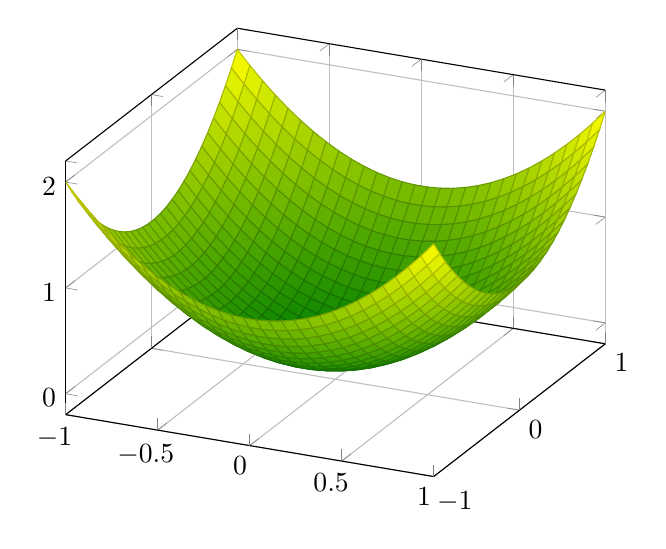
\begin{tikzpicture}\begin{axis}[grid=major,colormap/greenyellow]\addplot3[surf,samples=30,domain=-1:1]{x^2 + y^2};\end{axis}\end{tikzpicture}
% \end{center}
% Similarly there is a \nameref{local max} at $(0,0)$ for $z = -(x^2 + y^2)$.
% \begin{center}
%   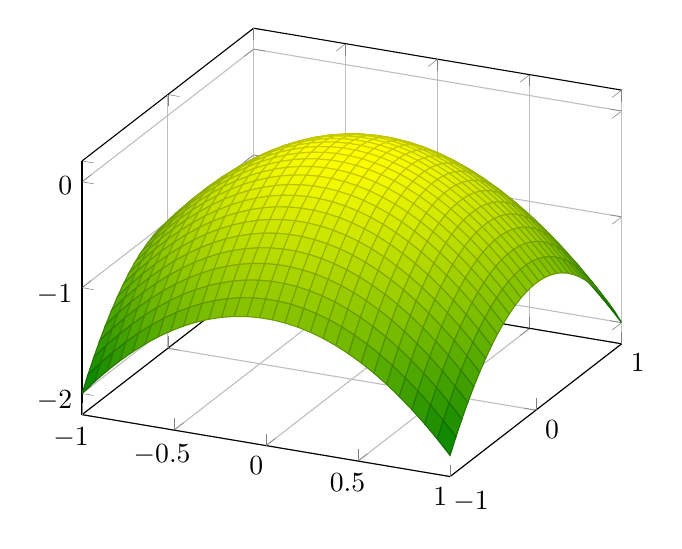
\begin{tikzpicture}\begin{axis}[grid=major,colormap/greenyellow]\addplot3[surf,samples=30,domain=-1:1]{-x^2 - y^2};\end{axis}\end{tikzpicture}
% \end{center}
% Additionally, for $f(x,y) = z = x^2 - y^2$ (Saddle Surfce) we have a \nameref{saddle point} at $(0,0)$.
% \begin{center}
%   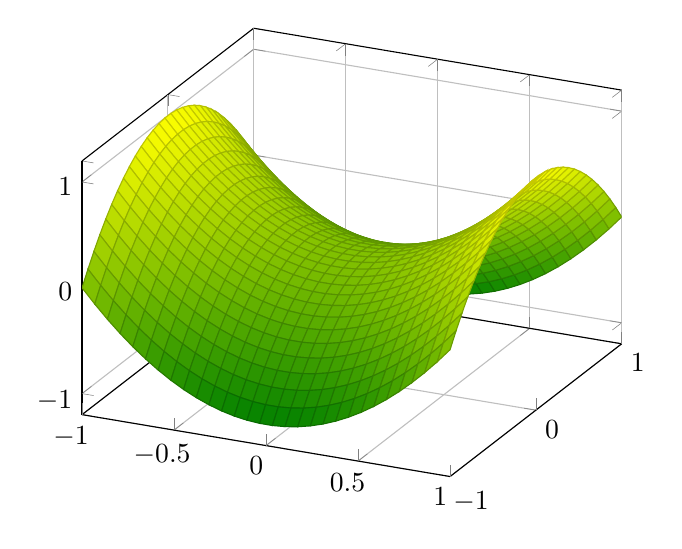
\begin{tikzpicture}\begin{axis}[grid=major,colormap/greenyellow]\addplot3[surf,samples=30,domain=-1:1]{x^2 - y^2};\end{axis}\end{tikzpicture}
% \end{center}
\[ f_x = 2x = 0 \]
\[ f_y = -2y = 0 \]
which implies that $(x,y) = (0,0)$ is a \nameref{critical point}.
\end{exmp}

\subsection{Finding Critical Points}

\begin{exmp}
  Suppose we have $f(x,y) = y^3 + x^2 - 6xy + 3x + 6y$. Find the \nameref{critical point}s. \\

  First we find where $f_x=0$ or DNE and $f_y = 0$ or DNE. Well,
  \begin{align*}
    f_x & = 2x - 6y + 3 = 0 \\
    f_y & = 3y^2 - 6x + 6 = 0
  \end{align*}
  Then rearrange the first equation to get $x = \f{3-6y}{2}$ and then plug into second equation to get $3y^2 - 6 \left( \f{3-6y}{2} \right) + 3 = 0$ which implies that $y = 1$ or $y = 5$. So, when $y = 1$, $x = \f{6(1) - 3}{2} = \f{3}{2}$ and when $y = 5$ we have $x = \f{6(5) - 3}{2} = \f{27}{2}$. Therefore, the critical points are
  \[ \left( \f{3}{2}, 1 \right) \ \ \ \ \mbox{ and } \ \ \ \ \left( \f{27}{2}, 5 \right)\]
\end{exmp}

\begin{exmp}
  Let $f(x,y) = 6xy^2 - 2x^3 - 3y^4$. Then
  \begin{align*}
    f_x & = 6y^2 - 6x^2 = 0 \implies (y-x)(y+x) = 0 \ \ \ \ (1) \\
    f_y & = 12xy - 12y^3 = 0 \implies y(x-y^2) = 0 \ \ \ \ (2)
  \end{align*}
  So Equation (2) implies $y = 0$ or $x = y^2$. So, \\
  \textbf{Case 1} ($y = 0$): Then $(0-x)(0+z) = 0$ by (1) which implies $x=0$. Therefore one \nameref{critical point} is $(0,0)$. \\
  \textbf{Case 2} ($x = y^2$): Then
  \begin{align*}
    (y+y^2)(y-y^2) = 0 \implies y^2(1 + y)(1-y) = 0 \implies y = 0,-1,1
  \end{align*}
  Then since $x = y^2$, $y = 0 \implies x = 0$, $y = -1 \implies x = (-1)^2 = 1$ and $y = 1 \implies x = 1^2 = 1$. Therefore we have that $(1,-1)$ and $(1,1)$ are also \nameref{critical point}s. We conclud that the \nameref{critical point}s are
  \[ \left( 0, 0 \right) \ \ \ \ \mbox{ and } \ \ \ \ \left( 1, -1 \right)  \ \ \ \ \mbox{ and } \ \ \ \ \left( 1, 1 \right) \]
\end{exmp}

\subsection{Classifying Critical Points}

If $f \in C^2$ and $(a,b)$ is a \nameref{critical point} of $f$ then
\[ f(x,y) \approx f(a,b) + \cancelto{0}{f_x(a,b)(x-a)} + \cancelto{0}{f_y(a,b)(y-b)} + \f{1}{2}\left( f_{xx}(a,b)(x-a)^2 + 2f_{xy}(a,b)(x-a)(y-b) + f_{yy}(a,b)(y-b)^2 \right) \]

\begin{defn}[quadratic form]\label{quadratic form}
A function of the form $Q(u,v) = a_{11}u^2 + 2a_{12}uv + a_{22}v^2$ is called a \textbf{quadratic form} on $\R^2$. In matrix form,
\[ Q(u,v) = (u,v)\left( \begin{matrix} a_{11} & a_{12} \\ a_{12} & a_{22} \end{matrix} \right) \left( \begin{matrix}
  u \\ v
\end{matrix} \right) \]
\end{defn}

\begin{defn}[positive definite]\label{positive definite}
If $Q(u,v) > 0$ for all $(u,v) \not = (0,0)$ then $Q$ is called a \textbf{positive definite}
\end{defn}
\begin{defn}[negative definite]\label{negative definite}
If $Q(u,v) < 0$ for all $(u,v) \not = (0,0)$ then $Q$ is called a \textbf{negative definite}
\end{defn}
\begin{defn}[indefinite]\label{indefinite}
If $Q(u,v) > 0$ for some $(u,v)$ and $Q(u,v) < 0$ for some other $(u,v)$, then $Q$ is called \textbf{indefinite}.
\end{defn}
\begin{defn}[semidefinite]\label{semidefinite}
If $Q$ is neither \nameref{positive definite}, \nameref{negative definite}, nor \nameref{indefinite} then $Q$ is called \textbf{semidefinite}. For example, $Q > 0$ for some $(u,v)$, and $Q = 0$ for some other $(u,v) \not = (0,0)$.
\end{defn}

\begin{exmp}
  Suppose $Q(x,y) = 3x^2 + y^2 > 0$ for all $(x,y) \not = (0,0)$, then $Q$ is \nameref{positive definite}.
\end{exmp}

\begin{exmp}
  Suppose $Q(x,y) = 3x^2 + 5xy +y^2$. Note $Q(x,0) = 3x^2 > 0$ and $Q(1,-1) = 3-5 + 1 < 0$ then by definition, $Q$ is \nameref{indefinite}.
\end{exmp}

\textbf{Comment:} The terminology also applies to the corresponding matrix. For eample, in Example 10.4, we say that
\[ \left( \begin{matrix}
  3 & 0 \\
  0 & 1
\end{matrix} \right) \]
is \nameref{positive definite}. Also, in Example 10.5, we say that
\[ \left( \begin{matrix}
  3 & \f{5}{2} \\
  \f{5}{2} & 1
\end{matrix} \right) \]
is \nameref{indefinite}.

\newcommand{\mtx}[1]{\left( \begin{matrix}
  #1
\end{matrix} \right)}

\begin{thrm}\label{matrixdef}
  Let
  \begin{align*}
    Q(x,y) & = a_{11}x^2 + 2a_{12}xy + a_{22}y^2 = (x,y)\left( \begin{matrix} a_{11} & a_{12} \\ a_{12} & a_{22} \end{matrix} \right) \comb{x}{y}
  \end{align*}
  and $D = \det \mtx{ a_{11} & a_{12} \\ a_{12} & a_{22} } = a_{11}a_{22}-a_{12}^2$. Then,
  \begin{itemize}
    \item[(i)] $Q$ is \nameref{positive definite} iff $D > 0$ and $a_{11} > 0$.
    \item[(ii)] $Q$ is \nameref{negative definite} iff $D > 0$ and $a_{11} < 0$.
    \item[(iii)] $Q$ is \nameref{indefinite} iff $D < 0$.
  \end{itemize}
  If $D = 0$, $Q$ is called \textbf{degenerate}, and is classified as \nameref{semidefinite}.
\end{thrm}

\begin{defn}[determinant]\label{determinant}
The \textbf{determinant} of a $2\times 2$ matrix $M = \mtx{a & b \\ c & d}$ is
\[ \det(M) = ad - bc \]
\end{defn}

\textbf{Back to Critical Points} \\

Near a \nameref{critical point} $(a,b)$, \[f(x,y) - f(a,b) \approx \f{1}{2} \left[ f_{xx}(a,b)(x-a)^2 + 2f_{xy}(a,b)(x-a)(y-b) + f_{yy}(a,b)(y-b)^2 \right] = ...\] assuming that $f \in C^2$. Well we the $\f{1}{2}$ doesn't matter much, and let's let $(x-a) = u$ and $(y-b) = v$, then
\[ ... = \f{1}{2} (u,v) \mtx{f_{xx}(a,b) & f_{xy}(a,b) \\ f_{xy}(a,b) & f_{yy}(a,b)} \comb{u}{v} \]
so this is why the \nameref{hessian} is useful, before this it was basically just a fancy name.

\begin{thrm}[second-derivative test]\label{second-derivative test}
  If $f \in C^2$ in some \nameref{neighbourhood} of \nameref{critical point} $(a,b)$ then
  \begin{itemize}
    \item[(i)] If $Hf(a,b)$ is \nameref{positive definite}, $(a,b)$ is a \nameref{local min} point.
    \item[(ii)] If $Hf(a,b)$ is \nameref{negative definite}, $(a,b)$ is a \nameref{local max} point.
    \item[(iii)] If $Hf(a,b)$ is \nameref{indefinite}, then $(a,b)$ is neither a \nameref{saddle point}.
    \begin{note}
      The \nameref{semidefinite} case must be looked at seperately.
    \end{note}
  \end{itemize}
\end{thrm}
\begin{proof}
  See proof in Section 9.3 of course notes (not required for course).
\end{proof}

\begin{exmp}
  Classify \nameref{critical point}s of $f(x,y) = 6xy^2 - 2x^3 - 3y^4$. From Example 10.3, we already found the \nameref{critical point}s to be $(0,0)$, $(1,-1)$, and $(1,1)$. The \nameref{hessian} is
  \[ Hf(x,y) = \mtx{f_{xx} & f_{xy} \\ f_{xy} & f_{yy}} = \mtx{-12x & 12y \\ 12y & 12x - 36y^2} \]
  So,
  \begin{align*}
    Hf(0,0) & = \mtx{0 & 0 \\ 0 & 0}
  \end{align*}
  which has determinant $D = 0$. So $Hf(0,0)$ is \nameref{semidefinite}, that is $(0,0)$ is a degenerate \nameref{critical point} and must be looked at seperately (Later).
  \[ Hf(1,1) = \mtx{-12 & 12 \\ 12 & -24} \implies \det(Hf(1,1)) = (-12)(-24) - 12^2 > 0 \]
  Also, the first entry is -12 which is less than 0, so $Hf(1,1)$ is \nameref{negative definite} (by \autoref{matrixdef}), and $(1,1)$ is therefore a \nameref{local max} point.
  \[ Hf(1,-1) = \mtx{-12 & -12 \\ -12 & -24} \implies \det(Hf(1,-1)) = (12)(24) - 12^2 > 0 \]
  since the first first entry is -12 which is less than 0, at $(1,-1)$ we also have a \nameref{local max}.\\

  \textbf{Back to $(0,0)$} \\

  $f(x,y) = 6xy^2 - 2x^3 - 3y^4$, then the question is whether $f(x,y) > 0$ or $f(x,y) < 0$ near $(0,0)$. Well, $f(x,0) = -2x^3$, which means that, by definition $(0,0)$ is a \nameref{saddle point}
\end{exmp}

\begin{exmp}
  Consider $f(x,y) = x^2y - 2xy^2 + 3xy + 4$, find and classify the \nameref{critical point}s. \\

  First,
  \[ f_x = 2xy - 2y^2 + 3y = y(2x - 2y + 3) = 0 \ \ \ \ \ \ \ (1) \]
  \[ f_y = x^2 - 4xy + 3x = x(x - 4y + 3) = 0 \ \ \ \ \ \ \ (2) \]
  (2) implies that $x = 0$ or $x - 4y + 3 = 0$. If $x = 0$ then equation (1) implies $y(-2y + 3) = 0$ which implies $y = 0$ or $\f{3}{2}$. \\

  Now, if $x - 4y + 3 = 0$, then $x = 4y - 3$, and equation (1) implies $y(2(4y-3) - 2y + 3) = 0$ implies $y = 0, \f{1}{2}$. Then, $x = -3$ or $-1$ respectively. Therefore the \nameref{critical point}s are
  \[ (0,0),\left( 0,\f{3}{2} \right), (-3,0), \left( -1, \f{1}{2} \right) \]
  Next, the \nameref{hessian} is
  \[ HF(x,y) = \mtx{2y & 2x - 4y + 3 \\ 2x-4y+3 & -4x} \]
  Then
  \[ |Hf(0,0)| = \left| \begin{matrix}
    0 & 3 \\ 3 & 0
  \end{matrix}\right| = -9 < 0\]
  so (0,0) is a \nameref{saddle point}. And,
   \[ |Hf(-3,0)| = \left| \begin{matrix}
    0 & -3 \\ -3 & 12
  \end{matrix}\right| = -9 < 0\]
  so (-3,0) is a \nameref{saddle point}. And,
  \[ \left| Hf \left( 0,\f{3}{2} \right) \right| = \left| \begin{matrix}
    3 & -3 \\ -3 & 0
  \end{matrix}\right| = -9 < 0\]
  is another \nameref{saddle point}. Finally,
  \[ \left| Hf \left( -1,\f{1}{2} \right)\right| =  \left| \begin{matrix}
    1 & -1 \\ -1 & 4
  \end{matrix}\right| = 4 - 1 = 3 > 0\]
  So $Hf \left( -1, \f{1}{2} \right)$ is \nameref{positive definite} and $\left( -1, \f{1}{2} \right)$ a \nameref{local min} point.
\end{exmp}

\begin{rem} \
  \begin{itemize}
    \item If $(a,b)$ is not a \nameref{critical point}, then $\nabla f(a,b) \not = (0,0)$ (assuming it exists). $(a,b)$ is called a \textbf{regular point} of $f$ and the \nameref{level curve}s are smooth around these points
    \item If $f \in C^2$ and $(a,b)$ is a non-degenerate (that is $|Hf(a,b)| \not = 0$), then $f(x,y) \approx P_{2,(a,b)}(x,y)$. The \nameref{level curve}s of $P_2$ will be approximately equal to the \nameref{level curve}s of $f$.  \end{itemize}
\end{rem}

\section{Extreme Values}

Given $f(x,y)$, how can we find the maximum and minimum values on $S \subset \R^2$?

\begin{defn}[abolute maximum point]\label{absolute maximum point}
If $f(\va) \geq f(\vx) \forall \vx \in S$ then $\va$ is an \textbf{absolute maximum point}; the value $f(\va)$ is the \textbf{absolute maximum value of $f$}.
\end{defn}


\begin{defn}[abolute minimum point]\label{absolute minimum point}
If $f(\va) \leq f(\vx) \forall \vx \in S$ then $\va$ is an \textbf{absolute minimum point}; the value $f(\va)$ is the \textbf{absolute minimum value of $f$}.
\end{defn}

Recall, to maximize a single variable function $f(x)$ on $[a,b]$, check critical points and end points. (Extreme Value Theorem) \\

\begin{defn}[boundary point]\label{boundary point}
  A point $\va$ is a boundary point if every \nameref{neighbourhood} around $\va$ contains at least one point in $S$ and one point not in $S$.
\end{defn}

\begin{defn}[bounded]\label{bounded}
$S \subseteq \R^2$ is \textbf{bounded} means it can be contained in some \nameref{neighbourhood $N$}.
\end{defn}

\begin{defn}[closed]\label{closed}
  $S \subset \R^2$ is \textbf{closed} means that it contains all of its boundary points.
\end{defn}

If $S \subset \R^2$ is \textbf{closed} and \textbf{bounded} and $f$ is \nameref{continuous} on $S$, then $\exists \vc_1, \vc_2 \in S$ such that
\[ f(\vc_1) \leq f(\vx) \leq f(\vc_2) \mbox { \ \ for all $\vx \in S$} \]
\begin{proof}
  Beyond scope.
\end{proof}

\textbf{Algorithm for Extreme Values} \\
\begin{itemize}
  \item[1.] Evaluate $f$ at all \nameref{critical point}s in $S$.
  \item[2.] Find the maximum and minimum values of $f$ on the boundary of $S$.
  \item[3.] Choose the points from step 1. and step 2. which give the maximum and minimum values.
\end{itemize}

\begin{exmp}
  Find the \nameref{absolute maximum point} and \nameref{absolute minimum point} of $f(x,y) = xy - x - y + 3$ on a triangular region contained by the points $(0,4), (0,0)$ and $(2,0)$. \\

  \begin{itemize}
    \item[1.] The \nameref{critical point}s:
    \begin{align*}
      f_x & = y - 1 = 0 \implies y = 1 \\
      f_y & = x - 1 = 0 \implies x = 1
    \end{align*}
    So the only \nameref{critical point} is $(1,1)$, and it is inside the triangle. Also,
    \[ f(1,1) = 2 \]

    \item[2.] The \nameref{boundary point}s are the points on the lines $x = 0$, $y = 0$, and $y = -2x + 4$. So,
    \begin{itemize}
      \item[i.] $x = 0, 0 \leq y \leq 4$ then $f(0,y) = -y + 3$ has maximum 3 and minimum -1.
      \item[ii.] $y = 0, 0 \leq x \leq 2$ then $f(x,0) = -x + 3$ has maximum 3 and minimum 1.
      \item[iii.] $y = -2x +4, 0 \leq x \leq 2$ then $f(x,-2x+4) = -2x^2 + 5x -1$. From first year calculus, find the maximum and minimum of $g(x) = -2x^2 + 5x - 1$ on $0 \leq x \leq 2$. Then, $\ub{g(0) = -1, g(2) = 1}_{\mbox{endpoints}}$, and $g \left( \f{5}{4} \right) = \f{17}{8}$ (critical point).
    \end{itemize}
    \item[3.] Compare all values and find that the maximum of $f$ is 3 and the minimum of $f$ is -1.
  \end{itemize}
\end{exmp}

\begin{exmp}
  Suppose we have $f(x,y) = xy$. Find the maximum and minimum of $f$ on $S = \{(x,y) \ | \ x^2 + y^2 \leq 1 \}$ (points within a unit circle). \\

  \begin{itemize}
    \item The \nameref{critical point}s are found first, so
    \begin{align*}
      f_x = y = 0 \implies y = 0 \\
      f_y = x = 0 \implies x = 0
    \end{align*}
    so the only \nameref{critical point} is $(0,0)$ which is in $S$, and $f(0,0) = 0$.
    \item Look at the boundary of the function ($x^2 + y^2 = 1$), one way is to set $y^2 = 1-x^2$, so $y = \pm \sqrt{1-x^2}$. The other way is to parameterize the circle ($0 \leq t \leq 2\pi$),
    \begin{align*}
      x(t) = \cos t \\
      y(t) = \sin t
    \end{align*}
    (then $x^2 + y^2 = \cos^2 t + \sin^2 t = 1$). The value of $f$ on the curve is
    \[g(t) =  f(x(t),y(t)) = f(\cos t, \sin t) = \cos t \cdot \sin t \]
    So we need to find the maximum and minimum of $g$ on $[0,2\pi]$. The critical points of $g$:
    \begin{align*}
      g'(t) & = (\cos t) (\cos t) + (-\sin t)(\sin t) \\
      & = \cos^2 t - \sin^2 t \\
      & = \cos 2t & \mbox{(Identity)}
      & = 0
    \end{align*}
    which resolves to $2t = \f{\pi}{2}, \f{3\pi}{2}, \f{5\pi}{2}, \f{7\pi}{2}$ (since $0 \leq 2t \leq 4 4\pi$) so $t = \f{\pi}{4}, \f{3\pi}{4}, \f{5\pi}{4}, \f{7\pi}{4}$. Thus the points for respective $t$ values are,
    \[ \left( \f{1}{\sqrt{2}}, \f{1}{\sqrt{2}} \right), \ \ \left( \f{-1}{\sqrt{2}}, \f{1}{\sqrt{2}} \right), \ \ \f{-1}{\sqrt{2}}, \f{-1}{\sqrt{2}} , \ \ \f{1}{\sqrt{2}}, \f{-1}{\sqrt{2}}\]
    Now we plug in these $t$ values,
    \begin{align*}
      g(0) & = 0 \\
      g(2\pi) & = 0 \\
      g \left( \f{\pi}{4} \right) & = \f{1}{2} \\
      g \left( \f{3\pi}{4} \right) & = \f{-1}{2} \\
      g \left( \f{5\pi}{4} \right) & = \f{1}{2} \\
      g \left( \f{7\pi}{4} \right) & = \f{-1}{2}
    \end{align*}
    Clearly $\f{1}{2}$ is the absolute maximum of $f$, and $\f{-1}{2}$ is the absolute minimum of $f$.
    \end{itemize}
\end{exmp}

\textbf{Question.} What if it's difficult to parameterize the boundary? \\

\textbf{Idea.} Think of the boundary curve as the \nameref{level curve} of a fucntion $g(x,y)$:
\[ g(x,y) = k \]
Set $\nabla f = \lambda \nabla g$ (where $\lambda$ is a constant), so they're parallel. \\

\textbf{Idea of Proof}: Parameterize the boundary by $(x(t),y(t))$; define $u(t) = f(x(t),y(t))$, then set $u'(t) = 0$, then $\nabla f \bullet (x'(t), y'(t)) = 0$. Where $(x'(t),y'(t))$ is a tangent vector to the curve, by \nameref{chain rule}. So $\nabla f$ is perpendicular to the boundary curve, so $\nabla f$ is parallel to $\nabla g$. (see page 115-116 for a rigorous proof).

\subsection{Method of Lagrange Multipliers}\label{lagrange}

To find the maximum and minimum of $f(x,y)$ subject to contraint $g(x,y) = k$, evaluate $f$ at all points $(a,b)$ which satisfy:
\begin{itemize}
  \item $\nabla f(a,b) = \lambda \nabla g(a,b)$ and $g(a,b) = k$.
  \item $\nabla g(a,b) = (0,0)$ and $g(a,b) = k$.
  \item $(a,b)$ is an endpoint of the curve $g(x,y) = k$.
\end{itemize}
Then, the maximum of $f$ is the largest value of $f$ is obtained from points found in $(i) - (iii)$ and the minimum of $f$ is the smallest of the points found in steps 1 - 3. \\

\textbf{Comments:} \\
\begin{itemize}
  \item Assumed $g \in C^1$.
  \item Condition $(i)$ is 3 equations, 3 unknowns ($a,b,\lambda$):
  \begin{align*}
    f_x(a,b)&  = \lambda g_x(a,b) \\
    f_y(a,b) & = \lambda g_y(a,b) \\
    g(a,b) & = k
  \end{align*}
  $\lambda$ is called a \textbf{Lagrange Multiplier}.
  \item If $g(x,y) = k$ is an unbounded curve, one must consider $\lim_{||(x,y)|| \ar \infty}$ for $(x,y)$ satisfying $g(x,y) = k$.
  \item Generalizes to $f(x_1,x_2,\ldots,x_n)$ easily.
\end{itemize}

\begin{exmp}Find the \nameref{absolute maximum point} of $f(x,y) = x^2 + y$ on the region $S = \{(x,y) \ | \ x^2 + y^2 \leq 4\}$. \\

\begin{itemize}
  \item[1.] Find \nameref{critical point}s of $f$ inside $S$.
  \begin{align*}
    f_x = 2x = 0 \implies x = 0 \\
    f_y = 1 = 0 \implies \mbox{false}
  \end{align*}
  There are no \nameref{critical point}s.
  \item[2.] Find the maximum of $f$ on the boundary $x^2 + y^2 \leq 4$. Let $g(x,y) = x^2 + y^2$ and let $k = 4$. Use Lagrange Multipliers with the constraint $g(x,y) = x^2 + y^2 = 4$.
  \begin{itemize}
    \item[i.] Set $\nabla f = \lambda \nabla g$, $g = 4$.
    \begin{align*}
      2x & = \lambda \cdot 2x & (1) \\
      1 & = \lambda \cdot 2y & (2) \\
      x^2 + y^2 & = 4 & (3)
    \end{align*}
    Equation (1) implies $\lambda = 1$ or $x = 0$. \\
    If $\lambda = 1$, then Equation (2) implies $y = \f{1}{2}$, and if $y = \f{1}{2}$ then $x = \pm \f{\sqrt{15}}{2}$. So this case gets
    \[ \left( \f{\sqrt{15}}{2}, \f{1}{2} \right) \]
    otherwise if $x = 0$, then by Equation (3), $y = \pm 2$, so another point is
    \[ (0,\pm 2) \]
    \item[ii.] Set $\nabla g = \vzero$, $g = 4$, then
    \begin{align*}
      2x & = 0 \\
      2y & = 0 \\
      x^2 + y^2 & = 4
    \end{align*}
    this system has no solution.
    \item[iii.] This equation has no endpoints (it's a circle).
  \end{itemize}
  \item[3.] Compare values:
  \[ f \left( \f{\sqrt{15}}{2}, \f{1}{2}  \right) = \left( \f{\sqrt{15}}{2} \right)^2 + \f{1}{2} = \f{17}{4} \]
  \[ f(0,2) = 0^2 + 2 = 2 \]
  \[ f(0,-2) = 0^2 -2 = -2 \]
  Therefore the absolute maximum value of $f$ is $\f{17}{4}$ and occurs at $ \left( \f{\sqrt{15}}{2}, \f{1}{2}  \right) $.
\end{itemize}
\end{exmp}

\begin{exmp}
  Let's say we have a Nuclear Reactor, and because we're doing applied math it is a cylinder with radius $r>0$ and height $h>0$, and has equation
  \[ \f{4}{r^2} + \f{\pi^2}{h^2} = k, \mbox{ \ \ \ a constant} \]
  Find the minimum volume of such a reactor. \\

  We want to minimize the volume, so first
  \[ f(r,h) = \pi r^2 h \]
  is the equation for volume of a cylinder, and it is subject to the contraint
  \[ \ub{\f{4}{r^2} + \f{\pi^2}{h^2}}_{g(r,h)} = k \]
  Using Lagrange Multipliers,
  \begin{itemize}
    \item[i.] Set $\nabla f = \lambda \nabla g$, and $g = k$, and $\nabla f = (f_r,f_h) = (2\pi r h, \pi r^2)$, and $\nabla g = \left( \f{-8}{r^3}, \f{-2\pi^2}{h^3} \right)$ so we get three equations,
    \begin{align*}
      2\pi r h & = \lambda \left( \f{-8}{r^3} \right) & (1)\\
      \pi r^2 & = \lambda \left( \f{-2\pi^2}{h^3} \right) & (2) \\
      \f{4}{r^2} + \f{\pi^2}{h^2}&  = k & (3)
    \end{align*}
    The first equation implies
    \[ \lambda = \f{-r^3 \pi r h}{4} = \f{-\pi}{4} r^4 h \]
    and the second implies
    \[ \lambda = \f{-r^2h^3}{2\pi} \]
    So,
    \begin{align*}
        \f{-\pi}{4} r^4 h & =  \f{-r^2h^3}{2\pi} \\
        r^2 & = \f{2h^2}{\pi^2}
    \end{align*}
    Pluging this $r^2$ into Equation 3 we get
    \[ \f{4}{\left( \f{2h^2}{\pi^2} \right)}  + \f{\pi^2}{h^2} = k \implies h = \sqrt{\f{3\pi^2}{k}} \implies r = \sqrt{\f{6}{k}} \]
    So one point is
    \[ \left( \sqrt{\f{6}{k}},  \sqrt{\f{3\pi^2}{k}} \right) \]
    \item[ii.] Set $\nabla g = 0$, $g = k$,
    \begin{align*}
      \f{-8}{r^3} & = 0 \\
      \f{-2\pi^2}{h^3} & = 0 \\
      \f{4}{r^2} + \f{\pi^2}{h^2}&  = k
    \end{align*}
    No points from this step (no solution).
    \item[iii.] What about endpoints of $\f{4}{r^2} = \f{\pi^2}{h^2} = k$? This curve is infinite, solving for $h$ describes the contraint curve
    \[ h = \f{\pi r}{\sqrt{kr^2 - 4}} \]
    which has an asymptote at $r = \f{2}{\sqrt{k}}$. So we should take a limit to get the "endpoint",
    \begin{align*}
       \lim_{r \ar \infty} f(r,h) & = \lim_{r \ar \infty} f \left( r, \f{\pi r}{\sqrt{kr^2 - 4}} \right) \\
       & = \lim_{r \ar \infty}\pi r^2 \left( \f{\pi r}{\sqrt{kr^2 - 4}} \right) \\
       & = \lim_{r \ar \infty} \f{\pi^2 r^2}{\sqrt{kr^2 - 4}} \\
       & = \lim_{r \ar \infty} \f{3\pi^2 r^2}{\f{1}{2} (2kr) (kr^2 - 4)^{-\f{1}{2}}} & \mbox{(L'Hopital's Rule)} \\
       & = \infty
     \end{align*}
     Similarly, $\displaystyle \lim_{h \ar \infty} f(r,h) = \infty$. So the minimum value is
     \begin{align*}
       f\left(  \sqrt{\f{6}{k}},  \sqrt{\f{3\pi^2}{k}} \right) & = \pi \f{6}{k} \sqrt{\f{3\pi^2}{k}} \\ & = \f{6\sqrt{3}\pi^2}{k^{\f{3}{2}}}
     \end{align*}
  \end{itemize}
\end{exmp}

\begin{exmp}
  Find the point(s) on the surface $z = xy + 5$ that are closest to the origin. \\

  We want to minimize distance from $(x,y,z)$ to the origin:
  \[ \sqrt{x^2 + y^2 + z^2} \]
  Better yet, minimize the squared distance, then take a square root at the end. So, minimize
  \[ f(x,y,z) = x^2 + y^2 + z^2 \]
  subject to contraint $\ub{z - xy}_{g(x,y,z)} = 5$. \\

  We use the Lagrange Multipliers Method:

  \begin{itemize}
    \item[(i)] Set $\nabla f = \lambda \nabla g$ and $g = 5$.
    \begin{align*}
      2x & = \lambda(-y) & (1) \\
      2y & = \lambda(-x) & (2) \\
      2z & = \lambda \cdot 1 & (3) \\
      z - xy & = 5 & (4)
    \end{align*}
    Then
    \[ \f{(1)}{(2)} \implies  \f{2x}{2y} = \f{-\lambda y}{-\lambda x} \mbox{if $x \not = 0$, $y \not = 0$} \]
    \begin{align*}
      \f{x}{y} & = \f{y}{x} \\
      x^2 & = y^2 \\
      y = \pm x \\
      \implies \lambda &= \f{2x}{-y} & (\mbox{from (1)}) \\
      \implies z & = \f{\lambda}{2} & (\mbox{from (2)})
    \end{align*}
    Putting this result into (4) gets
    \begin{align*}
      \f{-2}{2} - x(x) = -1 - x^2 = 5 & \mbox{(if $\lambda = -2$)} \\
       \f{2}{2} - x(-x) = 1 + x^2 = 5& \mbox{(if $\lambda = -2$)} \\
    \end{align*}
    The first case is impossible, and the second implies that $x^2 = 4$. So if $\lambda = 2 \implies y = -x$, and $z = \f{\lambda}{2} = 1.$ So our set is,
    \[ (2, -2), (-2, 2) \]
    What if $x = 0$ or $y = 0$? Then $z = 5$ from (4) and $\lambda = 10$ from (3) and thus $y = 0$ from (1) or (2). We get $(0,0,5)$.
    \item[(ii)] Set $\nabla g = 0$ and $g = 5$. Then
    \begin{align*}
      -y & = 0 \\
      -x & = 0 \\
      1 & = 0 \\
      z - xy & = 5
    \end{align*}
    Clearly no good, so there are no points from this approach.
    \item[(iii)] The boundary curve of the surface is $z - xy = 5$. Since the surface is unbounded, we check
    \[ \lim_{||(x,y,z)|| \ar \infty} f(x,y,z) =  \lim_{||(x,y,z)|| \ar \infty}  ||(x,y,z)||^2 = \infty \]
    which is clearly not a minimum. Then we check the points,
    \begin{align*}
      f(2,-2,1) & = 4 + 4 + 1 = 9 \\
      f(-2,2,1) & = 4 + 4 + 1 = 9 \\
      f(0,0,5) & = 0 + 0 + 5^2 = 25
    \end{align*}
    So the minimum squared disrance is 9 thus the minimum disrance is 3 for the points $(2,-2,1)$ and $(-2,2,1)$.
  \end{itemize}
\end{exmp}

\section{Coordinate Systems}

\begin{note}
  For this section, checking the course notes is more useful, since there's lots of sketches.
\end{note}

\begin{exmp}
  Convert to polar coordinates.
  \begin{itemize}
    \item[(a)] $x^2 + y^2 = 1$. So $r^2 = 1$, and so $r = 1$ (take $r > 0$). Which is a circle.
    \item[(b)] $x^2 + y^2 = \sqrt{x^2 + y^2} - x$. First,
    \begin{align*}
      r^2 & = r - r\cos \theta \\
      r & = 1 - \cos \theta \\
      \mbox{OR \ \ } r & = 0
    \end{align*}
    The $r = 0$ case is just a point on the origin, and otherwise the shape can be sketched as a "Cardioid" aka a heart.
  \end{itemize}
\end{exmp}

\begin{exmp}
  Find the area enclosed by Cardiois in the last example. \\

  "Cut up" $0 \leq \theta \leq 2\pi$ into increments of size $\Delta \theta$. Then the area is $\f{1}{2}r^2\Delta \theta = \f{1}{2} f(\theta)^2\Delta \theta$. We sum over all the $\theta$ calues and let $\Delta \theta \ar 0$. Then
  \begin{align*}
    A & = \int_0^{2\pi} \f{1}{2}(1-\cos \theta)^2 d \theta \\
    & = \f{1}{2} \int (1-\cancelto{0}{2\cos \theta} + \cos^2 \theta) d \theta \\
    & = \f{1}{2} (2\pi) + \f{1}{2} \int_0^{2\pi} \f{1}{2} + \f{\cancelto{0}{\cos (2\theta)}}{2} d\theta \\
    & = \f{3\pi}{2}
  \end{align*}
\end{exmp}

\subsection{Cylindrical Coordinates}

If we place the pole at the origin and the polar axis along the positive $x$-axis in polar coordinates and place the axis of symmetry along the $z$-axis we then can relate a point $P$ in cylindrical and Cartesian coordinates by
\begin{align*}
  x & = r\cos \theta \\
  y & = r\sin \theta \\
  z & = z
\end{align*}
and
\begin{align*}
  r & = \sqrt{x^2 + y^2} \\
  \tan \theta & = \f{y}{x} \\
  z & = z
\end{align*}

\begin{exmp}
  Consider the following
  \begin{itemize}
    \item[(a)] $r = 1$ represents a cylinder of radius 1.
    \item[(b)] $z = r$. Then,
    \begin{align*}
      z & = \sqrt{x^2 + y^2}
    \end{align*}
    which is a cone.
  \end{itemize}
\end{exmp}

\begin{exmp}
  Convert into cylindrical coordinates,
  \begin{itemize}
    \item[(a)] $z = xy$. Then
    \[ z = (r\cos \theta)(r\sin \theta) = r^2 \cos \theta \sin \theta = \f{1}{2}r^2 \sin 2\theta \]
    \item[(b)] $\ub{x^2 + y^2}_{r^2} + z^2 = 1$ which implies $z^2 = 1-r^2$ so $z = \pm \sqrt{1 -r^2}$. Th e best way to write it is probably $r^2 + z^2 = 1$.
  \end{itemize}
\end{exmp}

\subsection{Spherical Coordinates}

Let $\rho$ be the distance from a point to the origin, and like before the angle from the $x$-axis to the line projected by line from the origin is $\theta$, and the similar angle from the $z$-axis is $\phi$. That is, a point $P$ can be represented as $(\rho, \phi, \theta)$. Then,
\begin{align*}
  x&= \rho \sin \phi \cos \theta \\
  y & = \rho \sin \phi \sin \theta \\
  z & = \rho \cos \phi
\end{align*}
where $\rho \geq 0$ and $0 \leq \theta \leq 2 \pi$, and $0 \leq \phi \leq \pi$.

\begin{exmp}
  Discuss the points $(\rho, \phi, \theta) = \left( 1, \f{\pi}{2}. \f{\pi}{4} \right)$ and $\left( 2 , \pi, \f{3\pi}{4} \right)$ and convert to Cartesian.
  \begin{itemize}
    \item[(A)] $(x,y,z) = \left( 1\sin\f{\pi}{2}\cos\f{\pi}{4} ,1\sin\f{\pi}{2}\sin\f{\pi}{4} ,1\cos\f{\pi}{2} \right) = \left( \f{1}{\sqrt{2}}, \f{1}{\sqrt{2}}, 0 \right)$
    \item[(B)] $(x,y,z) = (0,0,2(-1)) = (0,0,-2)$.
  \end{itemize}
\end{exmp}
\begin{exmp}
  Some spherical coordinates:
  \begin{itemize}
    \item[(a)] $\rho = 1$ is sphere of radius 1.
    \item[(b)] $\phi = \f{\pi}{3}$ is a cone with every line having angle $\f{\pi}{3}$ with the origin vertical axis ($z$-axis).
    \item[(c)] Right $y>0$ half of the $yz$-plane
  \end{itemize}
\end{exmp}

\subsection{Mappings}

\begin{defn}[mapping]\label{mapping}
Consider $(u,v) = F(x,y) = (F_1(x,y), F_2(x,y))$. This is essentially like taking a point $(x,y)$ in a Domain $D$ on the $x-y$ plane and mapping it to some point $(u,v)$ in some other subset $R$ on the $u-v$ plane. This is called a "mapping" or "transformation".
\end{defn}

\begin{exmp}
  Find the image of $S = \{(x,y) \ | \ |x| \leq 1, |y| \leq 1 \}$ under the mapping
  \[ (u,v) = F(x,y) = (x+y, y) \]
  The region $S$ is just a square, where $x$ and $y$ are between -1 and 1. We can seperate this into four lines, for each side of the square, so
  \begin{align*}
   y & = 1 & -1 \leq x \leq 1 \\
   x & = 1 & -1 \leq y \leq 1 \\
   y & = -1 & -1 \leq x \leq 1 \\
   x & = -1 & -1 \leq y \leq 1
  \end{align*}
  The mapping is
  \begin{align*}
    u & = x + y \\
    v & = y
  \end{align*}
  Looking at the sides of the square:
  \begin{itemize}
    \item[(1)] $x = 1, -1 \leq y \leq 1$ implies
    \begin{align*}
      u & = 1 + y \\
      v & = y & -1 \leq v \leq 1
    \end{align*}
    \item[(2)] $y = 1, -1 \leq x \leq 1$ implies
    \begin{align*}
      u & = x + 1 & 0 \leq u \leq 2 \\
      v & = 1
    \end{align*}
  \end{itemize}
  You can keep doing this for the next two lines, and the resultant mapping on the $u-v$ plane is a parallelagram. Additionally, all inside points get mapped to the inside of the new shape.
\end{exmp}

Does the inside always necessarily get mapped to the inside of the new figure? The easiest way is to check a point inside $S$, say $(x,y) = (0,0)$ which implies $(u,v) = F(0,0) = (0,0)$. Yes, inside gets mapped to inside.

\begin{exmp}
  Consider the mapping
  \[ (x,y) = F(r,\theta) = (r\cos\theta, r\sin\theta) \]
  Find the image of $S = \{(r,\theta) \ | \ 0 \leq r \leq 1, 0 \leq \theta \leq \pi\}$.
  Again we clearly have a square region for $S$. \\

  \begin{itemize}
    \item Side 1: $\theta = \pi$ and $0 \leq r \leq 1$, which implies
    \begin{align*}
      x & = r\cos\theta = -r \\
      y & = r\sin\theta = 0
    \end{align*}
    which implies $y = 0$, $-1 \leq x \leq 0$.
    \item Side 2:
    \begin{align*}
      x & = 1\cos\theta \\
      y & = 1\sin\theta & 0 \leq \theta \leq \pi
    \end{align*}
    which implies $x^2 + y^2 = c^2 + s^2 = 1$. Which lies on a circle, and since $0 \leq \theta \leq \pi$, we have $\sin\theta \geq 0$ and $y \geq 0$, which is a semicircle.
    \item Side 3: $\theta = 0$, $0 \leq r \leq 1$ and
    \begin{align*}
      x & = r\cos0 = r \\
      y & = r\sin0 = 0
    \end{align*}
    so $y = 0$ with $0 \leq x \leq 1$ which closes off the semicircle.
    \item Side 4: $r = 0$, $0 \leq \theta \leq \pi$
    \begin{align*}
      x & = 0\cos\theta = 0 \\
      y & = 0\sin\theta = 0
    \end{align*}
    so $(x,y) = 0$ which is just one point, the origin.
  \end{itemize}
  Does the inside map to the inside? Try $(r, \theta) = \left( \f{1}{2}, \f{\pi}{2} \right)$ which implies $(x,y) = \left( \f{1}{2}\cos\f{\pi}{2}, \f{1}{2}\sin\f{\pi}{2} \right) = \left( 0, \f{1}{2} \right)$ which is inside the new shape. We're assuming that if one point maps from the inside to the inside, then they all do.
\end{exmp}

\subsection{Linear Approximation of a Mapping}

Say we have some point $(a,b)$ on the $xy$-plane, then the mapping $F$ will map this point to some other point $(c,d)$ in the $uv$-plane. Then the question is, will the point $(a+\Delta x, b+\Delta y)$ map to some other point $(c+\Delta u, d+\Delta v)$. \\

\textbf{Question.} How does a small change in $(x,y)$ affect $(u,v)$? \\

\textbf{Answer.} By \nameref{increment form} of the \nameref{linear approximation}, then thinking of $F(x,y) = (f(x,y), g(x,y))$ has $u = f(x,y)$ and $v = g(x,y)$ then
\[ \Delta u \approx f_x(a,b)\Delta x + f_y(a,b) \Delta y \]
and
\[ \Delta v \approx g_x(a,b)\Delta x + g_y(a,b) \Delta y \]
In matrix form:
\begin{align*}
  \comb{\Delta u}{\Delta v} & \approx \ub{\mtx{f_x(a,b) & f_y(a,b) \\ g_x(a,b) & g_y(a,b)}}_{DF(a,b)} \comb{\Delta x}{\Delta y} & DF(a,b) = \mbox{"derivative matrix"} \\
  \Delta \vu & \approx DF(\va) \Delta \vx \\
  F(\va + \Delta \vx) - F(\va) & \approx DF(\va)\Delta \vx \\
  F(\va + \Delta \vx) & \approx F(\va) + DF(\va)\Delta \vx
\end{align*}

\begin{exmp}
  Consider $F(x,y) = (x^2 + 2y, xe^y)$, estimate the image of the point $(2.01, -0.02)$. \\

  Use $(a,b) = (2,0)$. Then,
  \begin{align*}
    DF(x,y) & = \mtx{2x & 2 \\ e^y & xe^y} \\
    \implies DF(2,0) & = \mtx{4 & 2 \\ 1 & 2}
  \end{align*}
  So,
  \begin{align*}
    F(2,01, -0.02) & = F(2 + 0.01, 0 - 0.02) \\
    & \approx F(2,0) + DF(2,0) \mtx{0.01 \\ -0.02} \\
    & = \mtx{4 \\ 2} + \mtx{4 & 2 \\ 1 & 2} \mtx{0.01 \\ -0.02} \\
    & = \mtx{4 \\ 2} + \mtx{0 \\ -0.03} \\
    & = \mtx{4 \\ 1.97}
  \end{align*}
  so the image is approximately $(4, 1.97)$.
\end{exmp}

\subsection{Composite Mappings}

Suppose you have some point $(x,y)$ in the $xy$-plane and a mapping $G$ that maps it to some point $(u,v)$ into the $uv$-plane, and then some other mapping $F$ that maps this new point to the $pq$-plane then we can define a mapping that does both steps in one called $F \circ G$. \\

First apply the map $(u,v) = G(x,y)$ and then apply $(p,q) = F(u,v)$ to get the composite map $F\circ G(x,y)$ or $(p,q) = F(G(x,y))$. Then,
\begin{align*}
  F(G(x,y)) & = F(u(x,y), v(x,y)) \\
            & = (p(u(x,y), v(x,y)), q(u(x,y), v(x,y)))
\end{align*}

\textbf{Question.} How does the derivative matrix of $F\circ G$ relate to the derivative matricies of $F$ and $G$?

\begin{thrm}[chain rule in matrix form]\label{chainrulemtx}
If $G$ has \nameref{continuous} \nameref{partialderivative}s at $\vx = (x,y)$ and $F$ has \nameref{continuous} partials at $\vu = G(\vx)$ then $F\circ G$ has \nameref{continuous} partials at $\vx$ and
\begin{align*}
  D(F\circ G) & = DF(\vu) \cdot DG(\vx)
\end{align*}
\end{thrm}
\begin{proof}
  Note that $\f{\di q}{\di x} = \px \left( q(u(x,y), v(x,y)) \right)$, then we show
  \begin{align*}
    \mtx{ \f{\di p}{\di x} & \f{\di p}{\di y} \\ \f{\di q}{\di x} & \f{\di p}{\di y}} & = \mtx{\f{\di p}{\di u} & \f{\di p}{\di v} \\ \f{\di q}{\di u} & \f{\di q}{\di v}} \mtx{\f{\di u}{\di x} & \f{\di u}{\di y} \\ \f{\di v}{\di x} & \f{\di v}{\di y}}
  \end{align*}
  Then by the usual chain rule
  \begin{align*}
    \f{\di p}{\di x} & = \f{\di}{\di x} \left( p(u(x,y), v(x,y) \right) \\
    & = \f{\di p}{\di u} \f{\di u}{\di x} + \f{\di p}{\di v} \f{\di v}{\di x}
  \end{align*}
  which proves the first entry. The rest are similar.
\end{proof}

\begin{exmp}
  Find $D(F \circ G)$ where $F(u,v) = (u^2 + 2v, ue^v)$ and $G(x,y) = \left(\ub{y\cos x}_u, \ub{\f{\ln y}{x}}_v \right)$. \\

  By Chain rule,
  \begin{align*}
    D(F \circ G) & = DF(u,v) DG(x,y) \\
    & = \mtx{2u & 2 \\ e^v & ue^v} \mtx{-y\sin x & \cos x \\ \f{-\ln y}{x^2} & \f{1}{xy}} \\
    & = \mtx{-2uy\sin x - \f{2\ln y}{x^2} & 2u\cos x + \f{2}{xy} \\ -ye^v\sin x - \f{ue^v\ln y}{x^2} & e^v\cos x + \f{ue^v}{xy}} \\
    & = \cdots \mbox{(sub in $u = y\cos x$, $v = \f{\ln y}{x}$)}
  \end{align*}
\end{exmp}

\begin{exmp}
  Find $D(F \circ G)$ if $F(u,v) = (u\cos v, u\sin v)$ and $G(x,y) = \left( \sqrt{x^2 + y^2}, \arctan \left( \f{y}{x} \right) \right)$ where $x > 0$ and $y > 0$. \\

  By Chain Rule,
  \begin{align*}
    D(F\circ G) & = DF(u,v) DG(x,y) \\
    & = \mtx{\cos v & -u\sin v \\ \sin v & u\cos v} \mtx{\f{x}{\sqrt{x^2 + y^2}} & \f{y}{\sqrt{x^2 + y^2}} \\ \f{\left( \f{-y}{x^2} \right)}{1 + \left( \f{y}{x} \right)^2} & \f{\left( \f{1}{x} \right)}{1 + \left( \f{y}{x} \right)^2}} \\
    & = \mtx{\f{x\cos v}{\sqrt{x^2 + y^2}} + \f{yu\sin v}{x^2 + y^2}
              & \f{y\cos v}{\sqrt{x^2 + y^2}} - \f{xu\sin v}{x^2 + y^2}
              \\ \f{x\sin v}{\sqrt{x^2 + y^2}} +-\f{yu\sin v}{x^2 + y^2}
              & \f{y\sin v}{\sqrt{x^2 + y^2}} + \f{xu\cos v}{x^2 + y^2}}
  \end{align*}
  \begin{note}
    $u = \sqrt{x^2 + y^2}$ so $\f{u}{x^2 + y^2} = \f{1}{\sqrt{x^2 + y^2}}$, and $u = \arctan \left( \f{y}{x} \right) \implies \tan v = \f{y}{x}$ then by drawing the triangle to figure out other relations we see $\cos v = \f{x}{\sqrt{x^2 + y^2}}$, $\sin v = \f{y}{\sqrt{x^2 + y^2}}$. So plug in and simplify,
  \end{note}
  \begin{align*}
    D(F \circ G) & = \mtx{1 & 0 \\ 0 & 1}
  \end{align*}
  This mapping is essentially just converting from polar coordinates to cartesian, and then back. \\
  \textbf{Comment:} If we first subtitute
  \begin{align*}
    (F \circ G)(x,y) & = F(G(x,y)) \\
    & = F(\sqrt{x^2 + y^2}, \arctan \left( \f{y}{x} \right)) \\
    & = \left(\sqrt{x^2 + y^2}\cos \left( \arctan \left( \f{y}{x} \right) \right), \sqrt{x^2 + y^2}\sin \left( \arctan \left( \f{y}{x} \right) \right) \right) \\
    & = \left( \sqrt{x^2 + y^2} \f{x}{\sqrt{x^2 + y^2}}, \sqrt{x^2 + y^2} \f{y}{\sqrt{x^2 + y^2}} \right) \\
    & = (x,y)
  \end{align*}
  So
  \begin{align*}
    D(F\circ G) & = \mtx{\f{\di}{\di x}(x) & \f{\di}{\di y}(x) \\ \f{\di}{\di x}(y) & \f{\di}{\di y}(y)} \\
    & = \mtx{1 & 0 \\0 & 1}
  \end{align*}
\end{exmp}

\section{Inverse Mappings}

\begin{defn}[one-to-one]\label{one-to-one}
A \nameref{mapping} from $D_{xy}$ to $D_{uv}$ is \textbf{one-to-one} on $D_{xy} \subseteq \R^2$ if and only if
\[ F(a,b) = F(c,d) \implies (a,b) = (c,d) \]
for all $(a,b)$ and $(c,d) \in D_{xy}$.
\end{defn}

\begin{thrm}
  If $F$ is \nameref{one-to-one} on $D_{xy}$ then $F$ has an \textbf{inverse mapping} $F^{-1}$ such that \[(x,y) = F^{-1}(u,v) \iff (u,v) = F(x,y).\]
  Then we have $(F^{-1} \circ F)(x,y) = (x,y)$ $\forall (x,y) \in D_{xy}$.
\end{thrm}

\textbf{Question.} How do we determine if a given \nameref{mapping} is invertible?

We look at $DF(x,y)$.

\begin{thrm}
  Let $F$ be \nameref{one-to-one} on $D_{xy}$ with image $D_{uv}$ and inverse map $F^{-1}$. If $F$ has \nameref{continuous} \nameref{partialderivative}s at $(x,y) \in D_{xy}$ and $F^{-1}$ has \nameref{continuous} \nameref{partialderivative}s at $(u,v) = F(x,y)$ then
  \begin{align*}
    DF^{-1}(u,v))DF(x,y) & = I
  \end{align*}
\end{thrm}

\begin{proof}
  By earlier property,
  \begin{align*}
    (F^{-1} \circ F)(x,y) & = (x,y) \\
    \implies D(F^{-1}\circ F)(x,y) & = \mtx{1 & 0 \\  0 & 1} = I
  \end{align*}
  By \nameref{chainrulemtx},
  \begin{align*}
    D(F^{-1}\circ F)(x,y) & = I \\
    DF^{-1}(x,y) & = I
  \end{align*}
\end{proof}

\begin{itemize}
  \item So the derivative matrix is invertible if the \nameref{mapping} $F$ is invertible. Is the converse true? Does the derivative matrix being invertible imply that the mapping $F$ is invertible?
  \item How do you check if $DF$ is invertible? Show that the determinant is not zero.
\end{itemize}

\begin{defn}[Jacobian]\label{Jacobian}
The \textbf{Jacobian} of a \nameref{mapping}
\[ (u,v) = F(x,y) = (f(x,y), g(x,y)) \]
is denoted by
\[ \f{\di(u,v)}{\di (x,y)} \]
where
\begin{align*}
  \f{\di(u,v)}{\di(x,y)} & = \det(DF(x,y)) = \left| \begin{matrix} \pfx & \pfy \\ \f{\di g}{\di x} & \f{\di g}{\di y} \end{matrix} \right|
\end{align*}
\begin{note}
  If Theorem 13.2 holds, then $\det(DF^{-1}(u,v)DF(x,y)) = \det(I) = 1$, then
  \begin{align*}
    \f{\di(x,y)}{\di(u,v)} \cdot \f{\di(u,v)}{\di(x,y)} & = 1
  \end{align*}
  So,
  \[ \f{\di(u,v)}{\di(x,y)} = \f{1}{\f{\di(x,y)}{\di(u,v)}} \ \ \ \ \ \ \ \ \mbox{(inverse property)} \]
\end{note}
\end{defn}

\begin{exmp}
  Find the \nameref{Jacobian} of $G(x,y) = (\sqrt{x^2 + y^2}, \arctan \left( \f{y}{x} \right)$ \\

  \begin{align*}
    \jacu & = \det \mtx{\f{x}{\sqrt{x^2 + y^2}} & \f{y}{\sqrt{x^2 + y^2}} \\
                        \f{1}{1 + \left( \f{y}{x} \right)^2}\left( \f{-y}{x^2} \right) & 
                        \f{1}{1 + \left( \f{y}{x} \right)^2}\left( \f{1}{x} \right)} \\
         & = \mtx{\f{x}{\sqrt{x^2 + y^2}} & \f{y}{\sqrt{x^2 + y^2}} \\
                        \f{-y}{x^2 + y^2} & 
                        \f{x}{x^2 + y^2}} \\
        & = \f{x^2 + y^2}{(x^2 +y^2)^{\f{3}{2}}} \\
        & = \f{1}{\sqrt{x^2 + y^2}}
  \end{align*}
\end{exmp}

\begin{exmp}
  Same for $(x,y) = F(u,v) = (u\cos v, u\sin v)$.
  \begin{align*}
    \jacx & = \det \mtx{\cos v & -u\sin v \\ \sin v & u\cos v} \\
    & = u
  \end{align*}
  Notice that
  \[ \jacu \cdot \jacx = \f{1}{\sqrt{x^2 + y^2}}\cdot u = \f{1}{u} \cdot u, \ \ \ u \not = 0 \]
  Are the mappings inverses of each other? If $u = 0$, by inverse property not satisfied. By contrapositive of "F inverstible implies $\jacu \cdot \jacx = 1$" we get $F$ is not invertible at all points $(0, v)$ for any $v$. \\

  Note $(x,y) = F(0,v) = (0,0)$. Polar coordinates have a problem here! Are there any other $(u,v)$ "problem" points? If we plug in the point $(u, 2n \pi)$, then $F(u, 2n\pi + v_0) = F(u,v_0)$ so $F$ is not one-to-one so it is not invertible. \\

  The moral of the story is that we must restrict to neighbourhoods.
\end{exmp}

\begin{thrm}[Inverse Mapping Theorem]\label{inversemapping}
Let $(u,v) = F(x,y)$ where $u(x,y)$ and $v(x,y)$ have \nameref{continuous} \nameref{partialderivative}s at $(a,b)$. If $\jacu \not = 0$ at $(a,b)$ then there exists a \nameref{neighbourhood} of $(a,b)$ in which $F$ has an inverse mapping  $F^{-1}$ which has \nameref{continuous} \nameref{partialderivative}s.
\end{thrm}

\subsection{Inventing Mappings}

\begin{exmp}
  Invent a mapping that maps the ellipse $x^2 + 4xy + 5y^2 = 4$ onto the unit circle. Shwo that it is invertible and find the inverse. \\

  Then, $x^2 + 4xy + 5y^2 = 4 \implies (x+2y)^2 + y^2 = 4 \implies \left( \f{x+2y}{2} \right)^2 + \left( \f{y}{2} \right)^2 = 1$. Then let $u = \f{x+2y}{2}$ and $v = \f{y}{2}$ to get $u^2 + v^2 = 1$. Now we show that this mapping is invertible; The \nameref{Jacobian} is
  \begin{align*}
    \jacu & = \det \mtx{\f{1}{2} & 1 \\ 0 & \f{1}{2}} \\
          & = \f{1}{4} - 0 \\
          & = \f{1}{4} \\
          & \not = 0
  \end{align*}
  So there exists an inverse mapping on a \nameref{neighbourhood} of each point. To find the inverse of the entire mapping, we solve
  \begin{align*}
    v & = \f{x+2y}{2} \\
    v & = \f{y}{2}
  \end{align*}
  for $x$ and $y$. Well the second equation implies $v = 2v$ and then from the second get $x = 2u - 4v$.  So $F^{-1}$ is given by $(x,y) = F^{-1}(u,v) = (2u - 4v, 2v)$.
\end{exmp}

Note that for this example we didn't even need to calculate the \nameref{Jacobian} because just finding the inverse was enough. For more complicated $u$ and $v$ where we couldn't solve for $x$ and $y$ then we would rely more on the \nameref{Jacobian}.

\begin{exmp}
  Map a parallelogram with corners at $(-1,1)$, $(3,1)$, $(-3,-1)$ and $(1,-1)$ to a square. \\

  We have equations for all four sides, namely
  \begin{align*}
    y & = x - 2 \\
    y & = -1 \\
    y & = x + 2 \\
    y & = 1
  \end{align*}
  Let $v = y$, so $y = \pm 1$ implies $v = \pm 1$, this covers the two top and bottom straight lines already. Now for the other non-straight lines,
  \[ y = x - 2 \implies y - x = -2 \implies \f{y-x}{2} = -1 \]
  and
  \[ y = x + 2 \implies y - x = 2 \implies \f{y-x}{2} = 1 \]
  then let $u = \f{y-x}{2}$ to get lines $u = -1$ and $u = 1$. Next we check the point $(0,0)$ on the parallelogram, and it maps to the inside of the square also at $(0,0)$. So our conclusion is that
  \[ F(x,y) = (u,v) = \left( \f{y-x}{2}, y \right) \]
  maps the parallelogram to the square.
\end{exmp}

\textbf{Comment:} The \nameref{Jacobian} is
\begin{align*}
  \jacu & = \det \mtx{-\f{1}{2} & \f{1}{2} \\ 0 & 1} = -\f{1}{2}
\end{align*}
so by \nameref{inversemapping} there exists an inverse mapping around a neighbourhood of each point. Also, the area of the square is $2\times 2 = 4$ and the area of the parallelogram is $2\times 4 = 8$. Notice that they differ by a factor of a half.
\[ \f{1}{2} = \left| \f{-1}{2} \right| = \left| \jacu \right| \]
is the area scale factor. \\

Suppose we have some point $P =(x,y)$ that is the bottom left most corner of a rectangle with topleft corner $R$, and bottomright corner $Q$, then the topright corner is $(x + \Delta x, y + \Delta y)$ thus area $\Delta x \Delta y$.A mapping $F$ converts these all to $P' = (u,v)$, $R'$, $Q'$. Then the area of this nrw shape is approximately the area of the paralleogram for $\Delta x \Delta y$. Then the rectangle is formed by vertical line $PR$, and horizontal line $PQ$ which maps to the parallelogram with $P'R'$ and $P'Q'$. Then,
\[ PQ = \comb{\Delta x}{0} \implies P'Q' \approx \mtx{u_x & u_y \\ v_x & v_y} \comb{\Delta x}{0} = \comb{u_x \Delta x}{v_x \Delta x} \]
\[ PR = \comb{0}{\Delta y} \implies P'R' \approx \mtx{u_x & u_y \\ v_x & v_y} \comb{0}{\Delta y} = \comb{u_y \Delta y}{v_y \Delta y} \]

Then the area of our paralellogram is

\begin{align*}
  \left| \det \mtx{u_x\Delta x & u_y\Delta y \\ v_x\Delta x & v_y \Delta y} \right| & = \left| \det \mtx{u_x & u_y \\ v_x & v_y} \right|\Delta x \Delta y \\
  & = \left| \jacu \right| \Delta x \Delta y & \mbox{by definition}
\end{align*}

So the area of the image of the rectangle is approximately

\[ \left| \jacu \right| \Delta x \Delta y \]
and this is approximation becomes more accurate as $\Delta x, \Delta y \ar 0$. The \nameref{Jacobian} gives an "area scale factor".

\begin{exmp}
  Approximate the area of a small rectangle with $\Delta x \Delta y$ located at $(x,y) = (0,1)$ under the map $(u,v) = F(x,y) = (2x^2 + 2xy, y^2e^x)$. \\

  The \nameref{Jacobian} is 
  \[ \f{\di(u,v)}{\di(x,y)} = \det \mtx{4x + 2y & 2x \\ y^2e^x & 2ye^x} = \ub{\det \mtx{2 & 0 \\ 1 & 2}}_{\mbox{at $(0,1)$}} = 4 \]
  So the area of the image is $|4|\Delta x \Delta y = 4 \Delta x \Delta y$.
\end{exmp}

\textbf{Generalization.} $(u_1, u_2, \ldots, u_n) = F(x_1, x_2, \ldots, x_n)$. Then the derivative matrix is
\[ DF(x_1, \ldots, x_n) = \mtx{D_1F_1 & D_2F_1 & \cdots & D_nF_1 \\ D_1F_2 & D_2F_2 &  \cdots & D_nF_2 \\ \vdots & \vdots & \ddots & \vdots \\ D_1F_n & D_2F_n & \cdots & D_nF_n} \]
The \nameref{Jacobian} is
\[ \f{\di(u_1, u_2, \ldots, u_n)}{\di(x_1, x_2, \ldots, x_n)} = \det (DF) \]
If $n = 3$ then the absolute value of the \nameref{Jacobian} is the volume scale factor.

\begin{exmp}
  $(u,v,w) = F(x,y,z) = (xy,xz,yz)$. Then,
  \begin{align*}
    \f{\di(u,v,w)}{\di(x,y,z)} & = \det \mtx{y & x & 0 \\ z & 0 & x \\ 0 & z & y} \\
                               & = -xzy - yxz \\
                               & = -2xyz
  \end{align*}
\end{exmp}

For example, at point $(1,1,1)$ a rectangular prism (box) with volume $\Delta x \Delta y \Delta z$ would get mapped to a parallelpiped with volume $|-2(1)(1)(1)|\Delta x \Delta y \Delta z = 2\Delta x \Delta y \Delta z$.

\section{Double Integrals}

Recall from single variable functions,
\begin{align*}
  \int_a^b f(x) dx & = \lim_{\Delta x \ar 0} \sum_{i =1}^n f(x_i)\Delta x_i
\end{align*}
Then for $f(x,y)$ we consider some function $z = f(x,y)$ and we integrate over some region $D_{xy} \subseteq \R^2$ (think of a flat surface at $z = 0$). Imagine that we consider this domain as a grid being composed of some number of cells with width $\Delta x$ and heigh $\Delta y$. Then, suppose we turn each cell into a column of height $z = f(x,y)$. Then,
\newcommand{\Iint}{\iint\displaylimits}
\newcommand{\iintdxy}{\Iint_{D_{xy}}}
\begin{defn}[double integral]\label{doubleint}
\begin{align*}
  \iint\displaylimits_{D_{xy}} f(x,y) dx dy = \lim_{\substack{\Delta x \ar 0 \\ \Delta y \ar 0}} \sum_{i =1}^n f(x_1,y_i) \Delta x_i \Delta y_i
\end{align*}

We can interpret $\Iint_{D_{xy}} f(x,y) dA$ is the volume under a surface if $f > 0$. Additionally, $\Iint_{D_{xy}} 1 dA$ is the area of $D_{xy}$. Another example,
\[ \Iint_{D_{xy}} \rho (x,y) dA \]
where $\rho$ represents area density $(kg/m^2)$, then this double integral represents the totla mass of the plate. One more, suppose we want to calculate the average value of $f(x,y)$ over $D_{xy}$,
\[ f_{avg} = \f{\Iint_{D_{xy}}f(x,y) dA}{\Iint_{D_{xy}} 1 dA} \]
which is analogous to
\[ \f{\int_a^b f(x) dx}{b-a} = \f{\int_a^b f(x) dx}{\int_a^b 1 dx} \]

\end{defn}

\subsection{Evaluating $\Iint$}

\textbf{Key Idea.} Consider the cross-sections. Suppose we have some region $D_{xy}$, and we want to integrate over this area, starting from $x_l$ up to $x_u$, where the curve is closed for some lower function $y_l(x)$ and upper function $y_u(x)$. Then
\[ \iintdxy f(x,y) dA = \int_{x_l}^{x_u} \left( \ub{\int_{y_l(x)}^{y_u(x)} f(x,y) dy}_{\mbox{function of $x$}} \right) dx \]
called an "iterated integral". \\

\textbf{Another way.} Suppose we had another surface with two distinct curves that can be thought of with respect to $y$ like $x = x_u(x)$ on the right and $x = x_l(x)$ on the left. Then describe $D_{xy}$ by $y_l \leq y \leq y_u$ and $x_l(y) \leq x \leq x_u(y)$, then we can write
\[ \iintdxy f(x,y) dA = \int_{y_l}^{y_u} \left( \ub{\int_{x_l(y)}^{x_u(y)} f(x,y) dy}_{\mbox{function of $y$}} \right) dy \]

\begin{exmp}
  Evaluate $\Iint_D x^2 y dA$ where $D = \{(x,y) \ | \ 0 \leq x \leq 2, 0 \leq y \leq 1 \}$. \\

  \textbf{Solution.} One way:
  \begin{align*}
    \Iint_D x^2y dA & =  \int_0^2 \left( \int_0^1 (x^2y) dy\right)dx \\
                    & = \int_0^2 \left( x^2 \f{y^2}{2} \Big|_{y=0}^{y=1} \right) dx \\
                    & = \int_0^2 \left( \f{1}{2}x^2 - 0 \right) dx \\
                    & = \f{4}{3}
  \end{align*}
  Another way:
  \begin{align*}
    \Iint_D x^2y dA & = \int_0^1 \left( \int_0^2 x^2y dx \right) dy \\
                    & = \f{4}{3}
  \end{align*}
  \begin{note}Since $y$ is a constant with respect to $x$, and we have constant bounds, we could write
  \begin{align*}
    \int_0^1 \left( \int_0^2 x^2y dx \right) dy & = \int_0^1 \left( y \int_0^2 x^2 dx \right) dy \\
    & = \int_0^2 x^2 dx \int_0^1 y dy
  \end{align*}
  \end{note}
\end{exmp}

\begin{exmp} Let $D$ be bounded by $y = \sqrt{x}$ and $y = x^3$. Evaluate
\[ \Iint_D x^2 y^2 dA = I \]
\textbf{Solution.} First visualize this region as the the "cuban cigar" closed from $(0,0)$ to $(1,1)$ (the two intersecting points of the functions). We can describe $D$ as having $0 \leq x \leq 1$ and being careful about $y$, since it depends on the function values. The lower curve is $y = x^3$ and the upper curve is $y = \sqrt{x}$. Then, $x^3 \leq \sqrt{x}$. Now we can write it as an iterated integral,
\begin{align*}
  I & = \int_0^1 \left( \int_{x^3}^{\sqrt{x}} x^2y^2 dy \right) dx \\
    & = \mbox{(exercise)}
\end{align*}
Another way: Think of the region instead as horizontal strips, where $x = y^{\f{1}{3}}$ on the right and $x = y^2$ on the left, then $y^2 \leq x \leq y^{\f{1}{3}}$ and $0 \leq y \leq 1$. So,
\begin{align*}
  I & = \int_0^1 \left( \int_{y^2}^{y^{\f{1}{3}}} (x^2 y) dx \right) dy \\
    & = \int_0^1 \left( \f{x^3}{3} y^2 \Big|_{x = y^2}^{x = y^{\f{1}{3}}} \right) dy \\
    & = \int_0^1 \left( \f{y}{3}y^2 - \f{y^6}{3y^2} \right) dy \\
    & = \f{5}{108}
\end{align*}
\end{exmp}

\begin{exmp}
  Let $D$ be bounded by $y = x^2$ and $y = x + 2$. Find $\Iint_D (x + 2y) dA$. \\

  First make a sketch of both curves in the $xy$-plane, and figure out exactly which curve we're talking about. Then find the intersection points
  \begin{align*}
    x^2 & = x + 2 \\
    x^2 - x - 2 & = 0 \\
    x & = 2, -1
  \end{align*}
  So our region is between $-1$ and 2 and is bounded above by $y = x + 2$ and below by $y = x^2$. So,
  \begin{align*}
    \Iint_D (x + 2y) dA & = \int_{x = -1}^{x=2} \left(  \int_{y = x^2}^{y = x + 2} (x+2y) dy \right) dx \\
    & = \int_{-1}^2 \left( (xy + y^2) \big|_{y = x^2}^{y = x + 2} \right) dx \\
    & = \int_{-1}^2 (x(x+2) +(x+2)^2 - (x^3 + x^4)) dx \\
    & = \f{333}{20}
  \end{align*}

  \textbf{Comment.} Going the other way (integrating horizontally, not vertically): first we find the $y$ values of those two boundary values for $x$ (-1 and 2) and we get $(-1,1)$ and $(2,4)$. To get an idea of the problem, sketch the curve and notice that for $y$ values above $1$ we would be taking horizontal bars that on the left touch $y = x + 2$ whereas on the right they touch $y = x^2$. This is a bit of a problem, so we need to subdivide the two regions into $D_1$ (the lower one) and $D_2$ (the upper one).
  \begin{align*}
    \Iint_D (x+2y) dA & = \Iint_{D_1} (x+2y) dA + \Iint_{D_2} (x + 2y) dA \\
    & = \int_{y = 0}^{1} \left( \int_{-\sqrt{y}}^{\sqrt{y}} (x + 2y) dx \right) dy + \int_{y = 1}^{4} \left( \int_{y - 2}^{\sqrt{y}} (x + 2y) dx \right) dy \\
    & = \f{333}{20}
  \end{align*}
  \begin{itemize}
    \item So the shape of the region (partially) determines the order of integration
    \item Any other considerations?
  \end{itemize}
\end{exmp}

\begin{exmp}
  Evaluate $I = \Iint_D e^{y^2} dA$ where $D$ bounded by lines $x = 0$, $y = 1$ and $y = x$. (Again make a sketch, this region is a triangle). \\

  One way:
  \begin{align*}
    I & = \int_0^1 \left(\ub{\int_x^1 e^{y^2} dy}_{\mbox{impossible \frownie}} \right) dx
  \end{align*}

  Try the other order:
  \begin{align*}
    I & = \int_0^1 \left( \int_0^y e^{y^2} dx \right) dy \\
      & = \int_0^1 \left( \left[ e^{y^2}\right]  \Big|_{x = 0}^{x = y} \right) dy \\
      & = \int_0^1 \left( e^{y^2} y - 0 \right) dy \\
      & = \f{1}{2}e^{y^2}\Big|_0^1 \\
      & = \f{1}{2} \left( e -1  \right)
  \end{align*}
  \begin{itemize}
    \item So the integrand (the function in the $\Iint$) is also a consideration.
  \end{itemize}
\end{exmp}

\textbf{Properties of $\Iint$} \\

\textbf{Sum.} \[\Iint_D \left( f(x,y) + g(x,y) \right) dA  = \Iint_D f(x,y) dA + \Iint_D g(x,y)\]
\textbf{Scalar Multiple.} \[ \Iint_D kf(x,y) dA = k\Iint_D f(x,y) dA \]
\textbf{Inequality.} If $f(x,y) \leq g(x,y)$ for all $x, y \in D$ then
\[ \Iint_D f(x,y) dA \leq \Iint_D g(x,y) dA \]
\textbf{Triangle Inequality.} (absolute value inequality)
\[ \left| \Iint_D f(x,y) dA \right| \leq \Iint_D \left| f(x,y) \right| dA \]
\textbf{Decomposition Property.} If $D_1 \subseteq D$ and $D_2 \subseteq D$ and $D_1 \cap D_2 = \emptyset$ then
\[ \Iint_D f dA = \Iint_{D_1} f dA + \Iint_{D_2} f dA \]

\begin{thrm}[Change of Variable Theorem]\label{changevariablethrm}
\[ \iintdxy G(x,y) dxdy = \Iint_{D_{uv}} G(f(u,v), g(u,v)) \ub{\left| \f{\di(x,y)}{\di(u,v)}\right| dudv}_{dA} \]
where
\begin{itemize}
  \item $D_{xy}$ and $D_{uv}$ are closed, bounded sets with piecewise smooth boundary curve
  \item $(x,y) = F(u,v) = (f(u,v), g(u,v))$ is an invertible mapping of $D_{uv}$ onto $D_{xy}$ and $f \in C'$, $g \in C'$, $\jacx \not = 0$ on $D_{uv}$.
  \item $G(x,y)$ is \nameref{continuous} on $D_{xy}$.
\end{itemize}
\end{thrm}

\begin{exmp}
  Find $\Iint_D \f{1}{x^2 + y^2 + 1} dA$ on $D = \{ (x,y) \ | \ 4 \leq x^2 + y^2 \leq 16 \}$ \\

  This is a little complicated in Cartesian coordinates. The idea is to use polar coordinates to map to rectangle in the $r\theta$-plane. The mapping is
  \[ (x,y) = (r\cos\theta, r \sin\theta) \]
  and the \nameref{Jacobian} is
  \[ \jacx = \det \mtx{\cos \theta & -r\sin\theta \\ \sin\theta & r\cos\theta} = r\cos^2\theta -(-r\sin^2\theta) = r \]
  By \nameref{changevariablethrm},
  \begin{align*}
    \iintdxy  \f{1}{x^2 + y^2 + 1} dxdy & = \Iint_{D_{r\theta}}\f{1}{(r\cos\theta)^2 + (r\sin\theta)^2 + 1} \left|r \right| drd\theta \\
    & = \int_0^{2\pi} \left( \int_2^4 \f{r}{r^2 + 1} dr \right) d\theta \\
    & = \int_0^{2\pi} \f{1}{2} \ln(r^2 + 1) \Big|_2^4 d\theta \\
    & = \int_0^{2\pi} \left( \f{1}{2} \left( \ln 17 - \ln 5 \right) \right) d\theta \\
    & = \pi \ln \left( \f{17}{5} \right)
  \end{align*}
\end{exmp}

\begin{exmp}
  $\Iint_D y dA$ where $D = \{(x,y) \ | \ x^2 + y^2 \leq 2y\}$. \\

  First, $x^2 + y^2 \leq 2y \implies x^2 + (y-1)^2 \leq 1$. A clever way is to use modified polar coordinates:
  \[ (x,y) = (r\cos \theta, r \sin\theta + 1) \]
  $D_{r\theta}$ is described by $0 \leq r \leq 1$ and $0 \leq \theta \leq 2\pi$ so by \nameref{changevariablethrm}, (note that $\jacx = r$ still; shift of a constant doesn't affect the derivative matrix)
  \begin{align*}
    \Iint_D ydxdy & = \Iint_{D_{r \theta}} (r\sin\theta + 1) r drd\theta \\
    & = \int_0^{2\pi} \int_0^{1} (r^2\sin\theta + r) dr d\theta \\
    & = \int_0^{2\pi} \left( \f{1}{3} r^3 \sin\theta + \f{1}{2} r^2 \right) \Big|_0^1 d\theta \\
    & = \int_0^{2\pi} \left( \f{1}{3}\sin\theta + \f{1}{2} \right) d\theta \\
    & = \pi
  \end{align*}
\end{exmp}

\textbf{Comments.}

\begin{itemize}
  \item If we used "regular" polar $(x = r\cos\theta, y = r\sin\theta)$ then describe $D$ by $0 \leq \theta \leq \pi$ and $0 \leq r \leq 2\sin\theta$. Since $x^2 + y^2 \leq 2y$, $r \leq 2\sin\theta$ and we get
  \[ \int_0^{2\pi} \left( \int_0^{2\sin\theta} (\ub{r\sin\theta}_y) r dr \right) d\theta = ... \]
  \item The mapping is not invertible at the origin $(r = 0)$ - we ignore that since the value of an integral is not affected by only one point
\end{itemize}

\begin{exmp}
  Find $\iintdxy xydxdy$ where $D_{xy}$ is defined by the region enclosed by $y = x$, $y = x-1$, $y = -x$ and $y = -x + 2$ \\

  We can describe the lines differently,
  \[ x - y = 0 \ \ \ \ \ y = x - 1 \ \ \ \ \ x + y = 2 \ \ \ \ \ x + y = 0 \]
  The idea is to let $(u,v) = (x+y, x-y)$ and use \nameref{changevariablethrm}, and the answer is $\f{1}{4}$ (exercise)
\end{exmp}

\begin{exmp}
  $D_{xy}$ in the first quadrant is bounded by $xy = 1$, $xy = 2$, $x^2 - y^2 = 1$, $x^2 - y^2 = 2$. Evaluate $\iintdxy (x^2 + y^2) dA$. \\

  Let $u = x^2 - y^2$ and $v = xy$, then the region in the $uv$-plane is
  \[ \piecewise{1 \leq u \leq 2}{}{1 \leq v \leq 2}{} \]
  By the \nameref{changevariablethrm},
  \begin{align*}
    \iintdxy (x^2 + y^2) dA & = \Iint_{D_{uv}} ((x(u,v))^2 + (y(u,v))^2) \left| \jacx \right| du dv
  \end{align*}
  \begin{note}
    \[ \jacu = \det \mtx{2x & -2y \\ y & x} = 2(x^2 + y^2) \not = 0 \mbox{\ on $D_{xy}$ so $\exists$ an inverse mapping}  \]
    By inverse propery,
    \[ \jacx = \f{1}{\jacu} = \f{1}{2(x^2 + y^2)} \]
  \end{note}
  So,
  \begin{align*}
    \iintdxy (x^2 + y^2) dA & = \Iint_{D_{uv}} \cancel{(x^2 + y^2)} \left| \f{1}{2\cancel{(x^2+y^2)}} \right| du dv \\
    & = \f{1}{2}\int_1^2\int_1^2 dudv \\
    & = \f{1}{2}
  \end{align*}
\end{exmp}

\begin{exmp}[A famous integral]
  Evaluate
  \[ I = \int_0^{\infty} e^{-x^2} dx \]
  Multiply by $I$:
  \begin{align*}
    I^2 & =  \int_0^{\infty} e^{-x^2} dx \cdot  \int_0^{\infty} e^{-y^2} dy \\
    & = \int_0^{\infty} e^{-x^2} \left( \int_0^{\infty} e^{-y^2} dy \right) dx \\
    & = \int_0^{\infty} \left( \int_0^{\infty} e^{-(x^2 + y^2)} dy \right) dx
  \end{align*}
  Use polar coordinates:
  \[ \piecewise{x = r\cos\theta}{}{y = r\sin\theta}{}, \ \ \ \ \ \ \ \jacx = r \]
  So,
  \begin{align*}
    I^2 & = \int_0^{\f{\pi}{2}} \int_0^{\infty} e^{-r^2} \cdot |r| dr d\theta \\
        & = \int_0^{\infty}re^{-r^2}dr \int_0^{\f{\pi}{2}} \\
        & = -\f{1}{2}e^{-r^2}\Big|_0^{\infty} \cdot \theta \Big|_0^{\f{\pi}{2}} \\
        & = -\f{1}{2}(0 - 1)\f{\pi}{2} \\
        & = \f{\pi}{4}
  \end{align*}
  So \[ \int_0^{\infty} e^{-x^2} dx = \f{\sqrt{\pi}}{2} \]
\end{exmp}

\textbf{Comments:}

\begin{itemize}
  \item Technically an improper integral:
  \[ \int_0^{\infty}= \lim_{R \ar \infty} \int_0^R \]
  \item The "error function"
  \[ Erf(x) = \f{2}{\sqrt{\pi}}\int_0^x e^{-t^2}dt  \]
\end{itemize}

\section{Triple Intesdfgghjklbbnmwertuqazwsxedcrfvtgbyhnujmik,olp;/grals}
\newcommand{\Iiint}{\iiint\displaylimits}
Consider $f(x,y,z)$ and $D\subset \R^3$, slice $D$ into rectangular boxes, with volume $\Delta V_i = \Delta x_i \Delta y_i \Delta z_i$, and define

\begin{defn}[triple integral]\label{triple integral}
\[ \Iiint_D f(x,y,z) dv = \lim_{\substack{\Delta x_i \ar 0 \\ \Delta y_i \ar 0\\ \Delta z_i \ar 0}} \sum_{i =1}^n f(x_1,y_i,z_i) \Delta V_i \]
\end{defn}


\textbf{Interpretations.}

\[ \Iiint_d 1 dV = \mbox{\ volume of $D$} \]
\[ \Iint_D \ub{\rho(x,y,z)}_{\mbox{mass density}} dV = \mbox{\ the mass of $D$} \]

\[ \mbox{Average value of $f$ over $D$} = \f{\Iiint_D f(x,y,z) dV}{\Iint_D 1dv} \]

\subsection{Evaluating $\Iiint$}

Suppose we have some shape in $\R^3$ with some upper surface $z_u(x,y)$ and lower surface $z_l(x,y)$ over some region $D_{xy}$, then
\[ \Iiint_D f(x,y,z) dV = \iintdxy \left( \int_{z_l(x,y)}^{z_u(x,y)} f(x,y,z) dz \right) dxdy \]
$D$ is described by
\[ \piecewise{(x,y) \in D_{xy}}{}{z_l(x,y) \leq z \leq z_u(x,y)}{} \]

\begin{exmp}
  Find the mass of a tetrahedron formed by the planes $x = 0$, $y = 0$, and $z = 0$, and $\f{x}{a} + \f{y}{x} + \f{z}{c} = 1$, where the density is $\rho(x,y,z) = c - z$ $(a > 0, b> 0, c>0\ $ const) \\

  Mass $= \Iiint_D \rho(x,y,z) dV$ where $D$ is drawn in the book on page 15. $D$ is described by $0 \leq z \leq c \left( 1 - \f{x}{a} - \f{y}{b} \right)$ and $(x,y) \in D_{xy}$ has
  \[ \piecewise{0 \leq x \leq a}{}{0 \leq y \leq \f{-b}{a}x + b}{} \]
  So the mass is
  \begin{align*}
    m & = \Iiint_D (c-z) dV \\
      & = \iintdxy \left( \int_0^{c \left( 1 - \f{x}{a} - \f{y}{b} \right)} (c-z) dz \right) dxdy \\
      & = \f{1}{8} abc^2
  \end{align*}
\end{exmp}

\begin{exmp}
  Evalute $\Iiint_D \f{z}{4-x} dV$ where $D$ bounded by cylinder $x^2 + z^2 = 4$ and planes $x + y = 2$ and $2x + y= 6$, $z = 0$, and $z =0$ in the first octant. \\

  See textbook.
\end{exmp}

\begin{exmp}
  Find the volume of the region bounded by $z = x^2 + y^2$, $z = y + 2$. \\

  The volume is $\Iiint_D 1 dV$ where $D$ is drawn in class but here I'll just describe it; it's a cone.
\end{exmp}

If we only consider the $zy$-plane then it's just a parabola cut by $z= y + 2$, and since $z = x^2 + y^2$,
\[ x = \pm \sqrt{z - y^2} \]
so
\[-\sqrt{z - y^2} \leq x \leq \sqrt{z - y^2}  \]
So the volume is
\begin{align*}
  \Iiint_D 1 dV & = \Iint_{D_{yz}} \left( \int_{-\sqrt{z-y^2}}^{\sqrt{z-y^2}} 1 dx \right) dydz \\
  & = \int_{-1}^2 \left( \int_{y^2}^{y+2} \left( \int_{-\sqrt{z-y^2}}^{\sqrt{z-y^2}} 1 dx \right)dz \right) dy \\
  & = \int_{-1}^2 \left( \int_{y^2}^{y+2} \left( 2\sqrt{z-y^2} \right)dz \right) dy \\
  & = \int_{-1}^2 \left( \f{4}{3}(z-y^2)^{\f{3}{2}} \Big|_{y^2}^{y+2} \right) dy \\
  & = \f{4}{3} \int_{-1}^2 \left( \left( y + 2 - y^2 \right)^{\f{3}{2}} \right) dy
\end{align*}
Note that
\[ 2 - (y^2 - y) = 2 - \left( \left( y - \f{1}{2} \right)^2 - \f{1}{4} \right) = \f{9}{4} - \left( y - \f{1}{2} \right)^2 = \left( \f{3}{2} \right)^2 - \left( y - \f{1}{2} \right)^2 \]
also
\[ u = a\sin \theta \implies a^2 - u^2 = a^2 \cos^2\theta \]
so let $y - \f{1}{2} = \f{3}{2}\sin\theta$ so at $y = -1, \theta = \f{-\pi}{2}$ and $y = 2 \implies \theta = \f{\pi}{2}$, also $dy = \f{3}{2}\cos \theta$.
\begin{align*}
 & = \f{4}{3} \int_{-1}^2 \left( \left( y + 2 - y^2 \right)^{\f{3}{2}} \right) dy \\
  & = \f{4}{3} \int_{\f{\pi}{2}}^{-\f{\pi}{2}} \left( \left( \f{3}{2} \right)^2 - \left( \f{3}{2} \right)^2 \sin^2\theta \right)^{\f{3}{2}} \left( \f{3}{2}\cos\theta d\theta \right) \\
  & = \f{4}{2} \int_{\f{\pi}{2}}^{-\f{\pi}{2}} \left( \f{3}{2} \right)^2 (\cos \theta)^3 \f{3}{2} \cos \theta d \theta \\
  & = \f{27}{4} \int_{\f{\pi}{2}}^{-\f{\pi}{2}} \left( \cos^4 \theta d\theta  \right) \\
  & = \f{27}{4} \int_{\f{\pi}{2}}^{-\f{\pi}{2}} \left( \f{1}{2} + \f{1}{2} \cos 2\theta \right)^2 d\theta \\
  & = \f{81\pi}{32}
\end{align*}

\begin{thrm}[Change of Variable's Theorem]\label{changevariables}
  Let $(x,y,z) = F(u,v,w) = (f(u,v,w), g(u,v,w), h(u,v,w))$ and an invertible mapping of $D_{uvw}$ into $D_{xyz}$ with $f,g,h \in C^1$ and $\f{\di(x,y,z)}{\di(u,v,w)} \not = 0$ on $D_{uvw}$. If $G(x,y,z)$ is continuous on $D_{xyz}$ then
  \[ \Iiint_{D_{xyz}} G(x,y,z) dV = \Iiint_{D_{uvw}} G(f(u,v,w), g(u,v,w), h(u,v,w)) \left| \f{\di(x,y,z)}{\di(u,v,w)} \right| dudvdw \]
\end{thrm}

\begin{exmp}
  Find the volume in the first octant bounded by the hyperbolic cylinders $xy = 1$, $xy = 4$, $xz = 1$, $xz = 9$, $yz = 4$, $yz = 9$. \\

  Consider the mapping
  \[ (u,v,w) = F(x,y,z) \]
  given by
  \[ u = xy, \ \ \ \ \ \ v = xz \ \ \ \ \ \ w = yz \]
  then $D_{xyz}$ mapped to $D_{uvw}$ described by
  \[ 1 \leq u \leq 4 \ \ \ \ \ 1 \leq v \leq 9 \ \ \ \ \ 4 \leq w \leq 9 \]
  The \nameref{Jacobian}:
  \[ \f{\di(u,v,w)}{\di(x,y,z)} = \det \mtx{y & x & 0 \\ z & 0 & x \\ 0 & z & y} = -2xyz \]
  so
  \[ \f{\di(x,y,z)}{\di(u,v,w)} = \f{1}{-2xyz} = \f{-1}{2\sqrt{u}\sqrt{v}\sqrt{w}} \]
  By \nameref{changevariables},
  \begin{align*}
    V & = \Iiint_{D_{xyz}} 1 dV \\
      & = \Iiint_{D_{uvw}} 1 \left| \f{\di(x,y,z)}{\di(u,v,w)} \right|  dudvdw \\
      & = \int_1^4 \int_1^9 \int_4^9 \left( \f{1}{2\sqrt{u}\sqrt{v}\sqrt{w}} \right) dudvdw \\
      & = 8
  \end{align*}
\end{exmp}

\begin{exmp}
  Show tht the volume of a sphere of radius $R$ is $\f{4}{3} \pi R^3$. Consider the sphere centered at the orgiin $D_{xyz} = \{(x,y,z) \ | \ x^2 + y^2  + z^2 \leq R^2\}$. \\

  Converting to spherical coordinates:
  \[ D_{\rho \theta \phi} = \{(\rho, \theta, \phi) \ | \ 0 \leq \rho \leq R, 0 \leq \theta \leq 2\pi, 0 \leq \phi \leq \pi \} \]
  Then
  \begin{align*}
    V & = \Iint_{D_{xyz}} 1 dV \\
      & = \Iint_{D_{\rho \theta \phi}} 1 \left| \f{\di(x,y,z)}{\di(\rho, \theta, \phi)}  \right| dV \\
      & = \int_{\rho = 0}^R \int_{\theta =0}^{2\pi} \int_{\phi = 0}^{\pi} \rho^2 \sin \phi d\phi d\theta d\rho \\
      & = \f{4}{3} \pi R^3
  \end{align*}
\end{exmp}

\begin{exmp}
  Find the volume of an ice cream cone. (region bounded below by $z = \sqrt{x^2 = y^2}$ and above by $x^2 + y^2 + z^2 = z$). \\

  From the intersection of surfaces, $z = \sqrt{x^2 + y^2} \implies z^2 = x^2 + y^2$. Plug into the sphere equation and we get $2z^2 = z$ which implies $z = 0$ or $2z = 1 \implies z = \f{1}{2}$. First note that,
  \begin{align*}
    x^2 + y^2 + z^2 & = z \\
    x^2 + y^2 + \left( z^2 - z + \f{1}{4} \right) & = \f{1}{4} \\
    x^2 + y^2 + \left( z - \f{1}{2} \right)^2 & = \left( \f{1}{2} \right)^2
  \end{align*}Try spherical coordinates:
  \begin{align*}
    z & = \sqrt{x^2 + y^2} \\
   \rho \cos \phi & = \sqrt{(\rho \sin \phi \cos \theta)^2 + (\rho \sin \phi \sin \theta)^2} \\
   & = \sqrt{\rho^2 \sin^2 \phi} \\
   & = \rho \sin \phi \\
   1 & = \tan \phi \implies \phi = \f{\pi}{4}
  \end{align*}
  Then
  \begin{align*}
    x^2 + y^2 + z^2 & = z \\
    \rho^2 & = \rho \cos \phi \\
    \rho & = \cos \phi
  \end{align*}
  Also,
  \[ D_{\rho \theta \phi} = \{(\rho, \theta, \phi) \ | \ 0 \leq \rho \leq \cos \phi, 0 \leq \theta \leq 2\pi, 0 \leq \phi \leq \f{\pi}{4}\} \]
  \begin{align*}
    V & = \Iiint_{D_{xyz}} 1 dV \\
    & = \Iiintt_{D_{\rho \theta \phi}} 1 \left| \f{\di(x,y,z)}{\di(\rho, \theta, \phi)} \right| dV \\
    & = \int_{\theta = 0}^{2\pi} \int_{\phi=0}^{\f{\pi}{4}} \int_{\rho = 0}^{\cos \phi} \rho^2 \sin \phi d\rho d\phi d\theta
  \end{align*}
\end{exmp}

\end{document}
